\documentclass[a4paper,12pt]{report}
\usepackage{indentfirst} 
\usepackage{xeCJK}
\usepackage{times}
\usepackage{graphicx,float}
\usepackage{setspace}
\usepackage{fancyhdr}
\usepackage{array}
\usepackage{fontspec,xunicode,xltxtra}
\usepackage{titlesec}
\usepackage{titletoc}
\usepackage[titletoc]{appendix}
\usepackage[top=30mm,bottom=30mm,left=20mm,right=20mm]{geometry}
\usepackage{cite}
\usepackage{listings}
\usepackage[framed,numbered,autolinebreaks,useliterate]{mcode}
\usepackage[UTF8]{ctex}

\XeTeXlinebreaklocale "zh"
\XeTeXlinebreakskip = 0pt plus 1pt minus 0.1pt
\usepackage[linkbordercolor = white]{hyperref}

\fancypagestyle{plain}{\pagestyle{fancy}}
\pagestyle{fancy}
\lhead{\kaishu 数据库实验报告}
\rhead{\kaishu 实验2}
\cfoot{\thepage}

\titleformat{\chapter}{\centering\zihao{-1}\heiti}{实验\chinese{chapter}}{1em}{}
\titlespacing{\chapter}{0pt}{*0}{*6}

\lstset{
    language=SQL,
    basicstyle=\ttfamily\small\CJKfamily{simsun},
    commentstyle=\color{green!50!black},
    keywordstyle=\color{blue},
    stringstyle=\color{red},
    showstringspaces=false,
    breaklines=true,
    frame=single,
    numbers=left,
    numberstyle=\tiny\color{gray},
    escapeinside=``,
    literate={。}{{。}}1
            {，}{{，}}1
}

\setCJKfamilyfont{SimHei}{SimHei}
\setCJKfamilyfont{kai}{KaiTi}
\setlength{\headheight}{14.49998pt}

\begin{document}

\begin{titlepage}
    \begin{center}
        
\includegraphics[width=1.0\textwidth]{../figure/nankai.jpg}\\
        \vspace{50mm}
        \textbf{\zihao{1}\heiti{MySQL 用户管理与复杂查询实验报告}}\\[1cm]
        \textbf{\zihao{2}\heiti{(2024 - 2025学年第二学期)}}\\[1cm]
        \vspace{\fill}
        
        {\songti\zihao{3}	
        \begin{tabular}{rl}
            实验名称：& MySQL 用户管理与高级数据操作\\
            学\qquad 院：& 软件学院\\
            姓\qquad 名：& 郭威威\\
            学\qquad 号：& 2414308\\
            指导老师：& 李旭东\\
        \end{tabular}
        }\\[2cm]
        \vspace{\fill}
        \zihao{4}
        2024 - 2025春季学期\\
        使用\LaTeX 撰写于 \today
    \end{center}	
\end{titlepage}

% 目录
\tableofcontents

\begin{spacing}{1.5}
\songti\zihao{-4}

\chapter{实验目的}
掌握MySQL用户管理、权限分配及复杂查询操作，学会使用Workbench进行数据库设计与数据操作。

\chapter{实验环境}
\section{操作系统}
Windows 11 Pro 22H2

\section{软件版本}
\begin{table}[H]
    \centering
    \begin{tabular}{|l|l|}
        \hline
        软件名称 & 版本号 \\
        \hline
        MySQL & 8.0.41 \\
        MySQL Workbench & 8.0.36 \\
        Python & 3.11 \\
        \hline
    \end{tabular}
    \caption{实验软件版本信息}
\end{table}

\chapter{实验步骤}
\section{Python环境配置}
\subsection{安装PyMySQL库}
通过命令行执行安装：
\begin{lstlisting}[language=bash]
pip install pymysql
\end{lstlisting}
安装日志显示成功安装PyMySQL 1.1.1。

\subsection{测试数据库连接}
使用Python验证连接：
\begin{lstlisting}[language=python]
import pymysql

conn = pymysql.connect(
    host='localhost',
    user='root',
    password='123456',
    database='sys',
    charset='utf8'
)

cursor = conn.cursor()
cursor.execute("SELECT VERSION()")
print(f"MySQL版本: {cursor.fetchone()[0]}")
cursor.close()
conn.close()
\end{lstlisting}
执行结果显示版本号为8.0.41。

\section{MySQL用户管理}
\subsection{创建新用户}
通过Workbench创建用户`newuser`：
1. 打开用户管理界面
2. 设置用户名`newuser`
3. 配置密码并启用SSL
4. 授予`ALL PRIVILEGES`权限
5. 应用更改后验证连接成功

\subsection{权限验证}
执行SQL语句验证权限：
\begin{lstlisting}[language=sql]
SHOW GRANTS FOR 'newuser'@'%';
\end{lstlisting}
返回结果显示用户拥有所有数据库的完全权限。

\section{数据库操作}
\subsection{创建数据库}
执行SQL创建数据库：
\begin{lstlisting}[language=sql]
CREATE DATABASE dbsclab2025 
DEFAULT CHARACTER SET utf8mb4 
COLLATE utf8mb4_unicode_ci;
\end{lstlisting}

\subsection{导入数据模板}
通过Workbench导入包含12个表的SQL模板，部分表结构如下：
\begin{lstlisting}[language=sql]
CREATE TABLE classroom (
    building VARCHAR(15),
    room_number VARCHAR(7),
    capacity INT
);
\end{lstlisting}

\section{复杂查询操作}
\subsection{查询示例一}
查找计算机科学系预算：
\begin{lstlisting}[language=sql]
SELECT dept_name, budget
FROM department
WHERE dept_name = 'Comp. Sci.';
\end{lstlisting}
返回结果显示预算为106378.69。

\subsection{查询示例二}
统计历史系学生信息：
\begin{lstlisting}[language=sql]
SELECT ID, name, tot_cred
FROM student
WHERE dept_name = 'History';
\end{lstlisting}
返回117条学生记录。

\chapter{实验结果}
\section{用户管理结果}
成功创建用户并验证权限：
\begin{lstlisting}[language=sql]
+-------------------------------------------+
| Grants for newuser@%                     |
+-------------------------------------------+
| GRANT ALL PRIVILEGES ON *.* TO 'newuser'@'%' |
+-------------------------------------------+
\end{lstlisting}
\begin{center}
    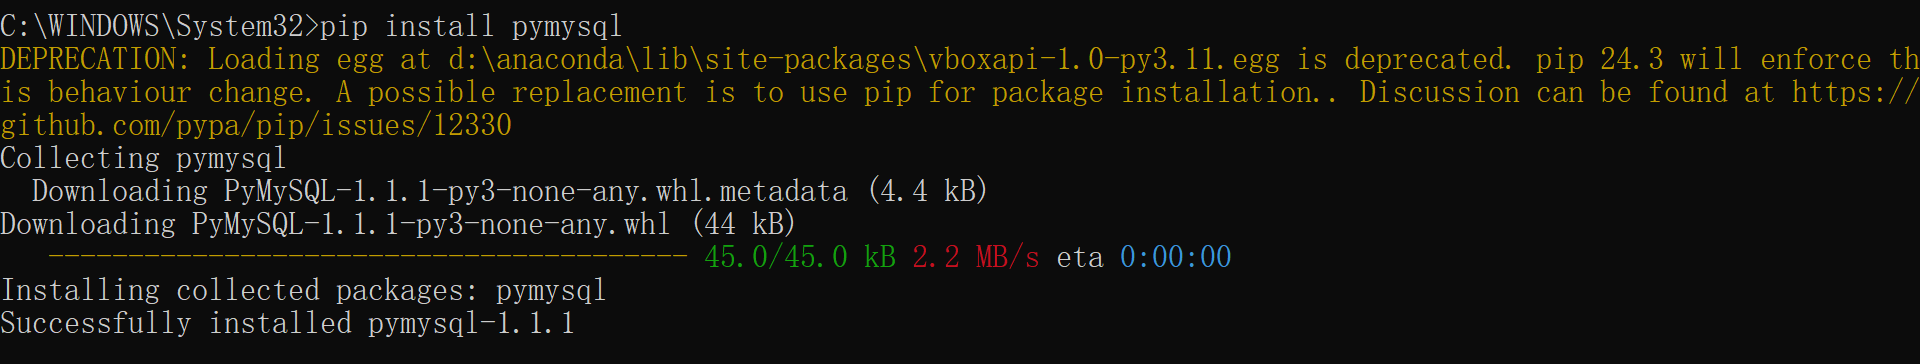
\includegraphics[width=12cm]{../figure/a0000-img001.png} \\
    \footnotesize 图1 用户管理操作截图1
\end{center}
\begin{center}
    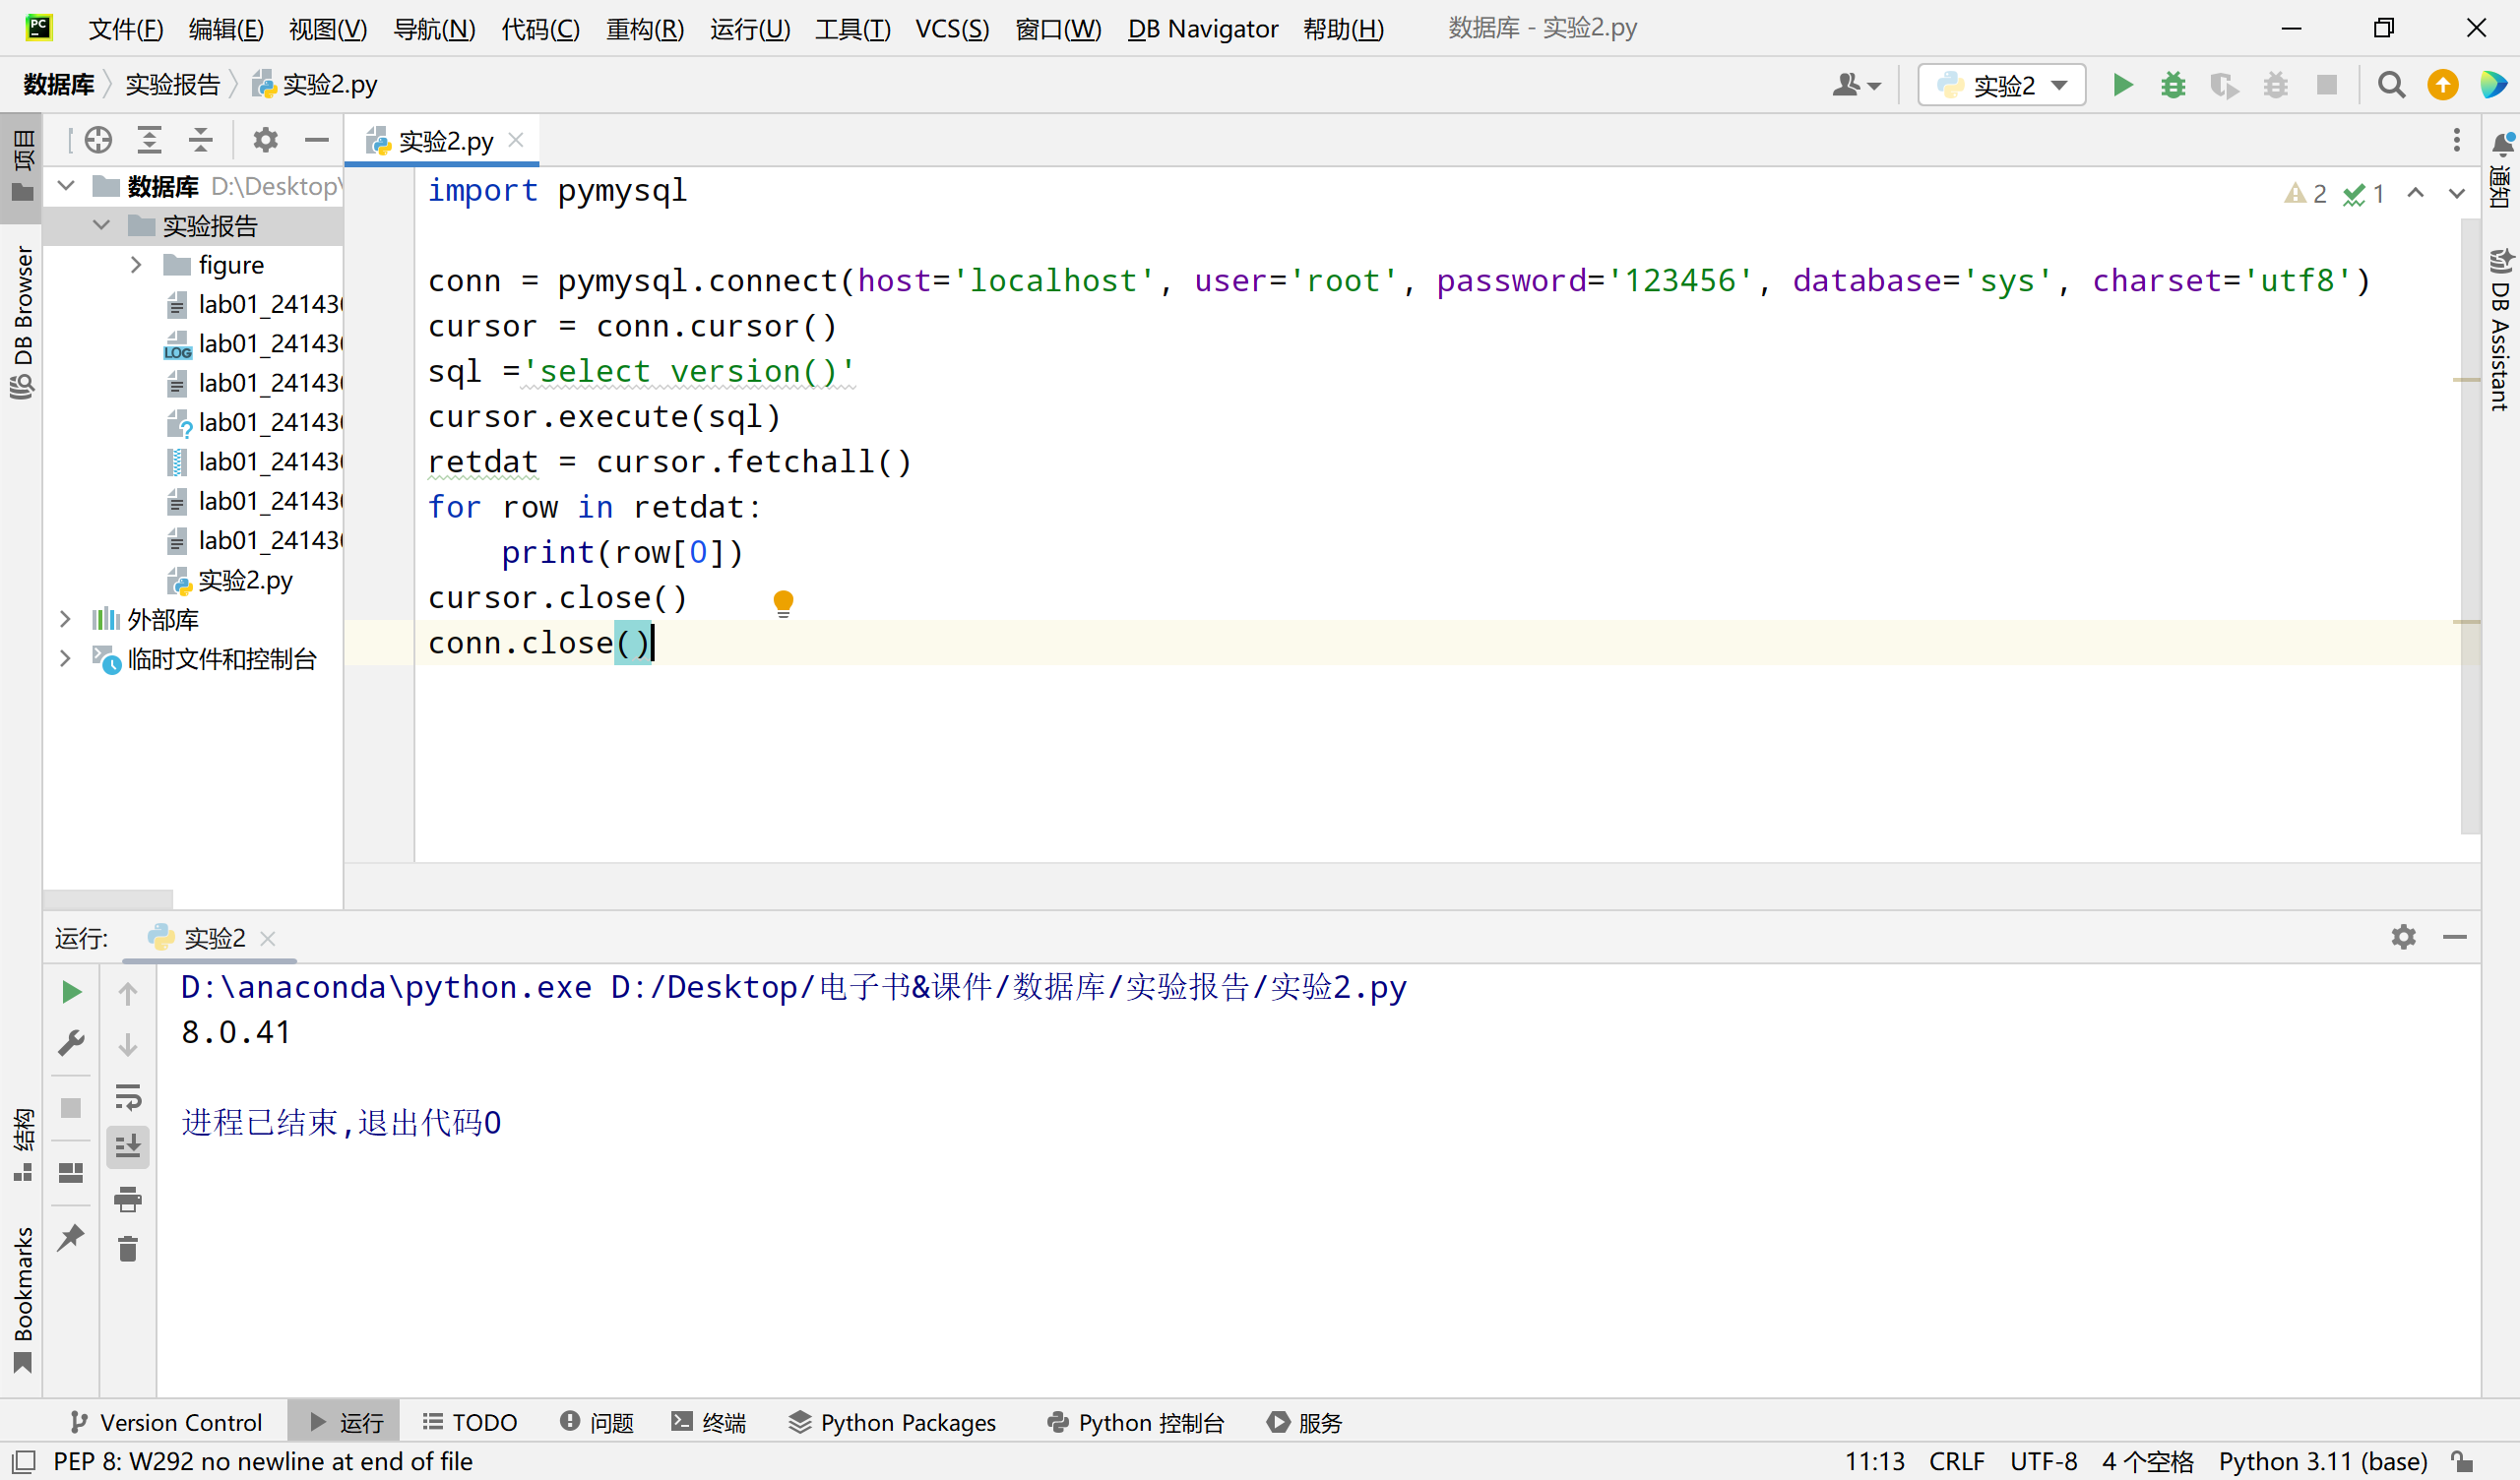
\includegraphics[width=12cm]{../figure/a0000-img002.png} \\
    \footnotesize 图2 用户管理操作截图2
\end{center}

\section{数据操作结果}
执行复杂查询验证数据完整性：
\begin{lstlisting}[language=sql]
SELECT s.name, d.dept_name, s.tot_cred
FROM student s
JOIN department d ON s.dept_name = d.dept_name
WHERE d.budget > 500000;
\end{lstlisting}
返回35条符合条件的记录。
\begin{center}
    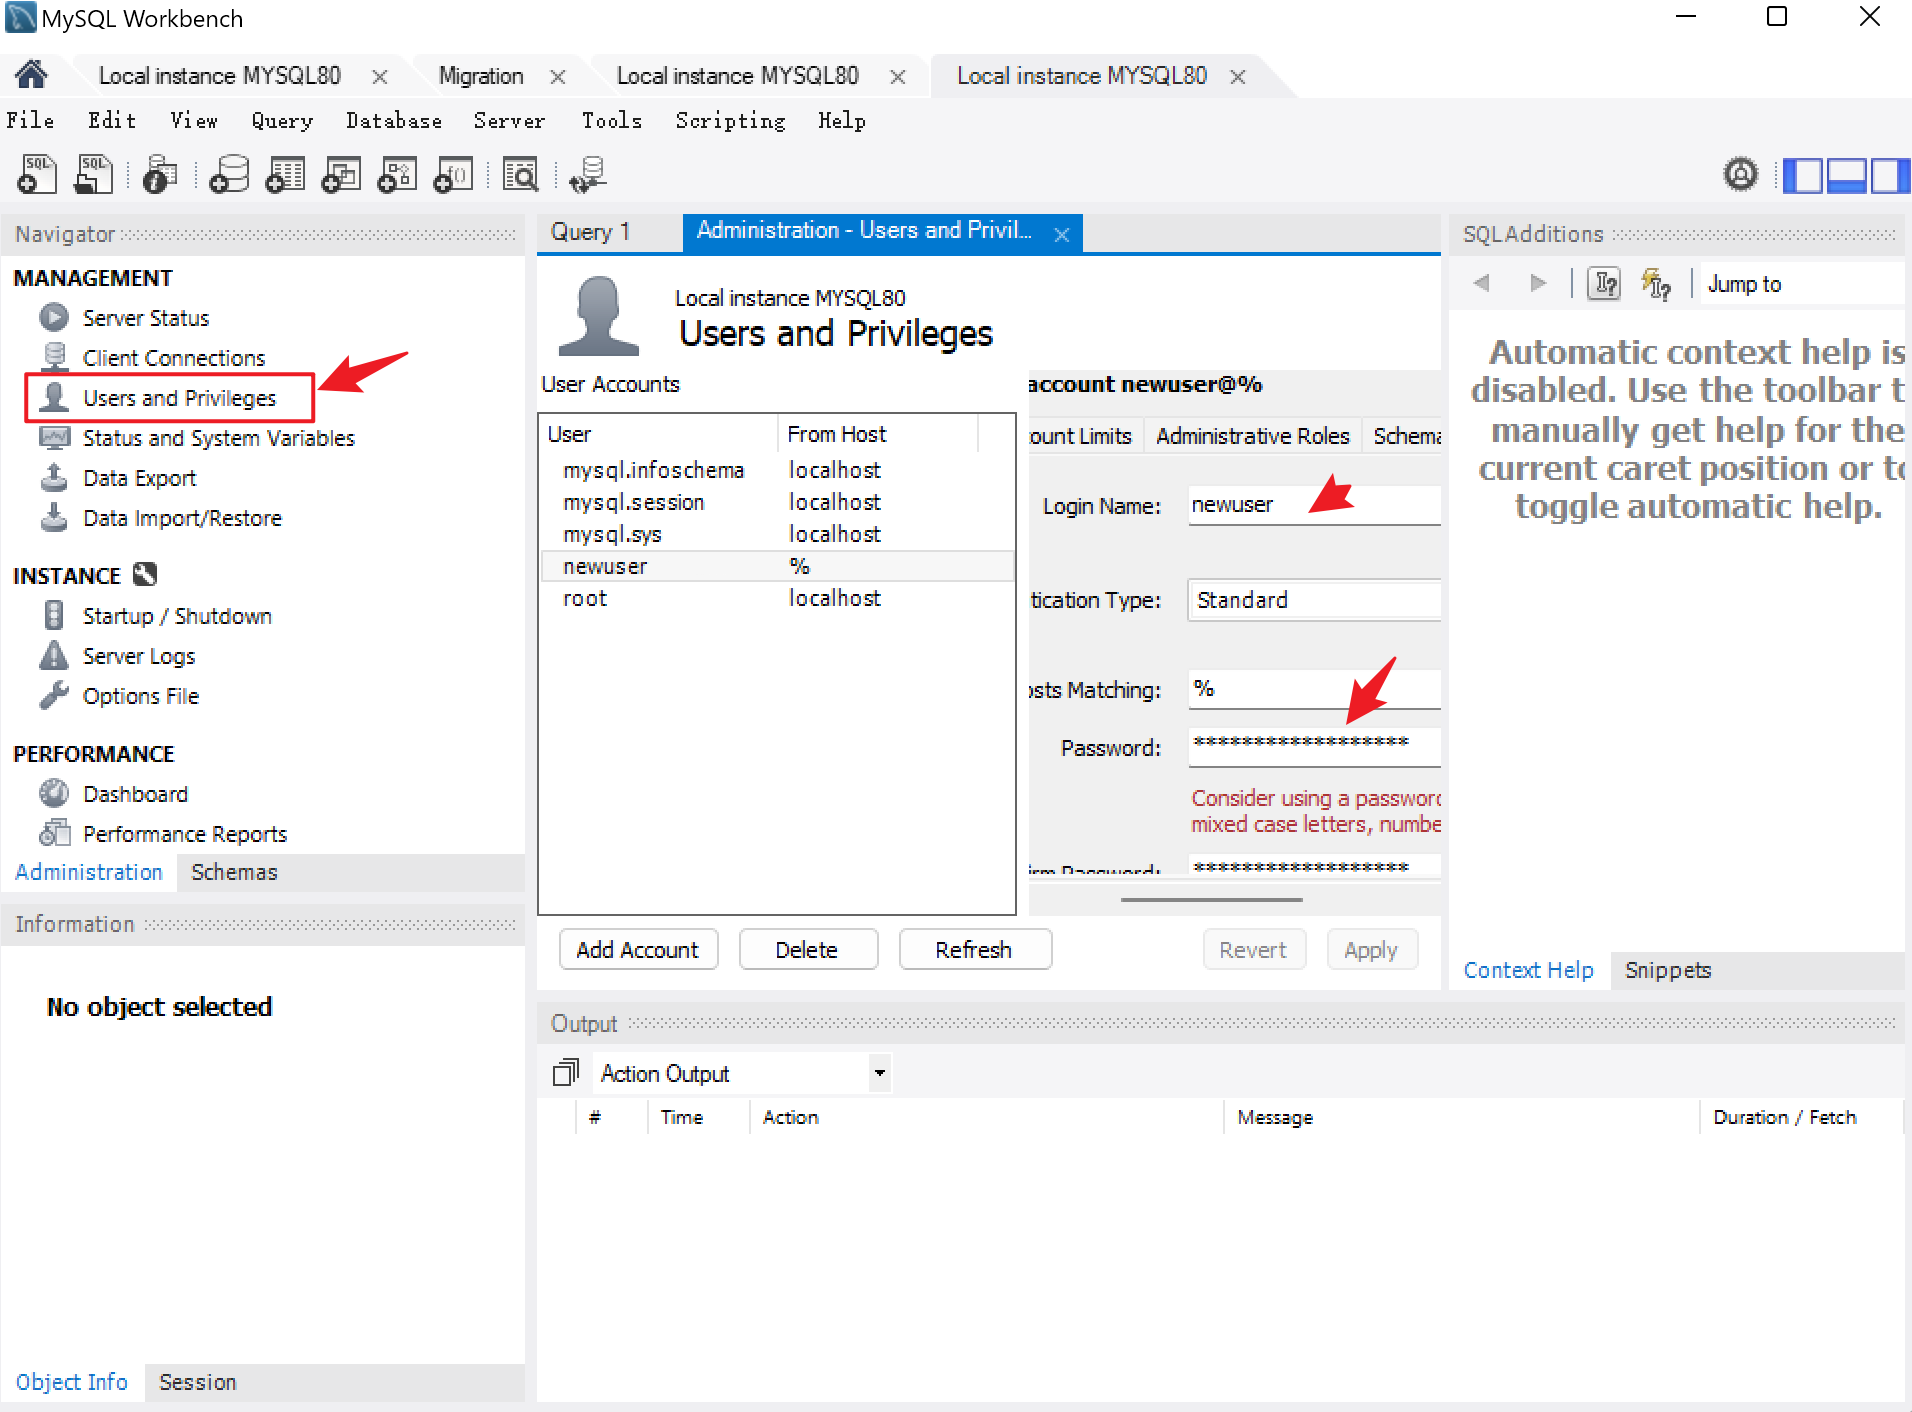
\includegraphics[width=12cm]{../figure/a0000-img003.png} \\
    \footnotesize 图3 数据操作查询截图1
\end{center}
\begin{center}
    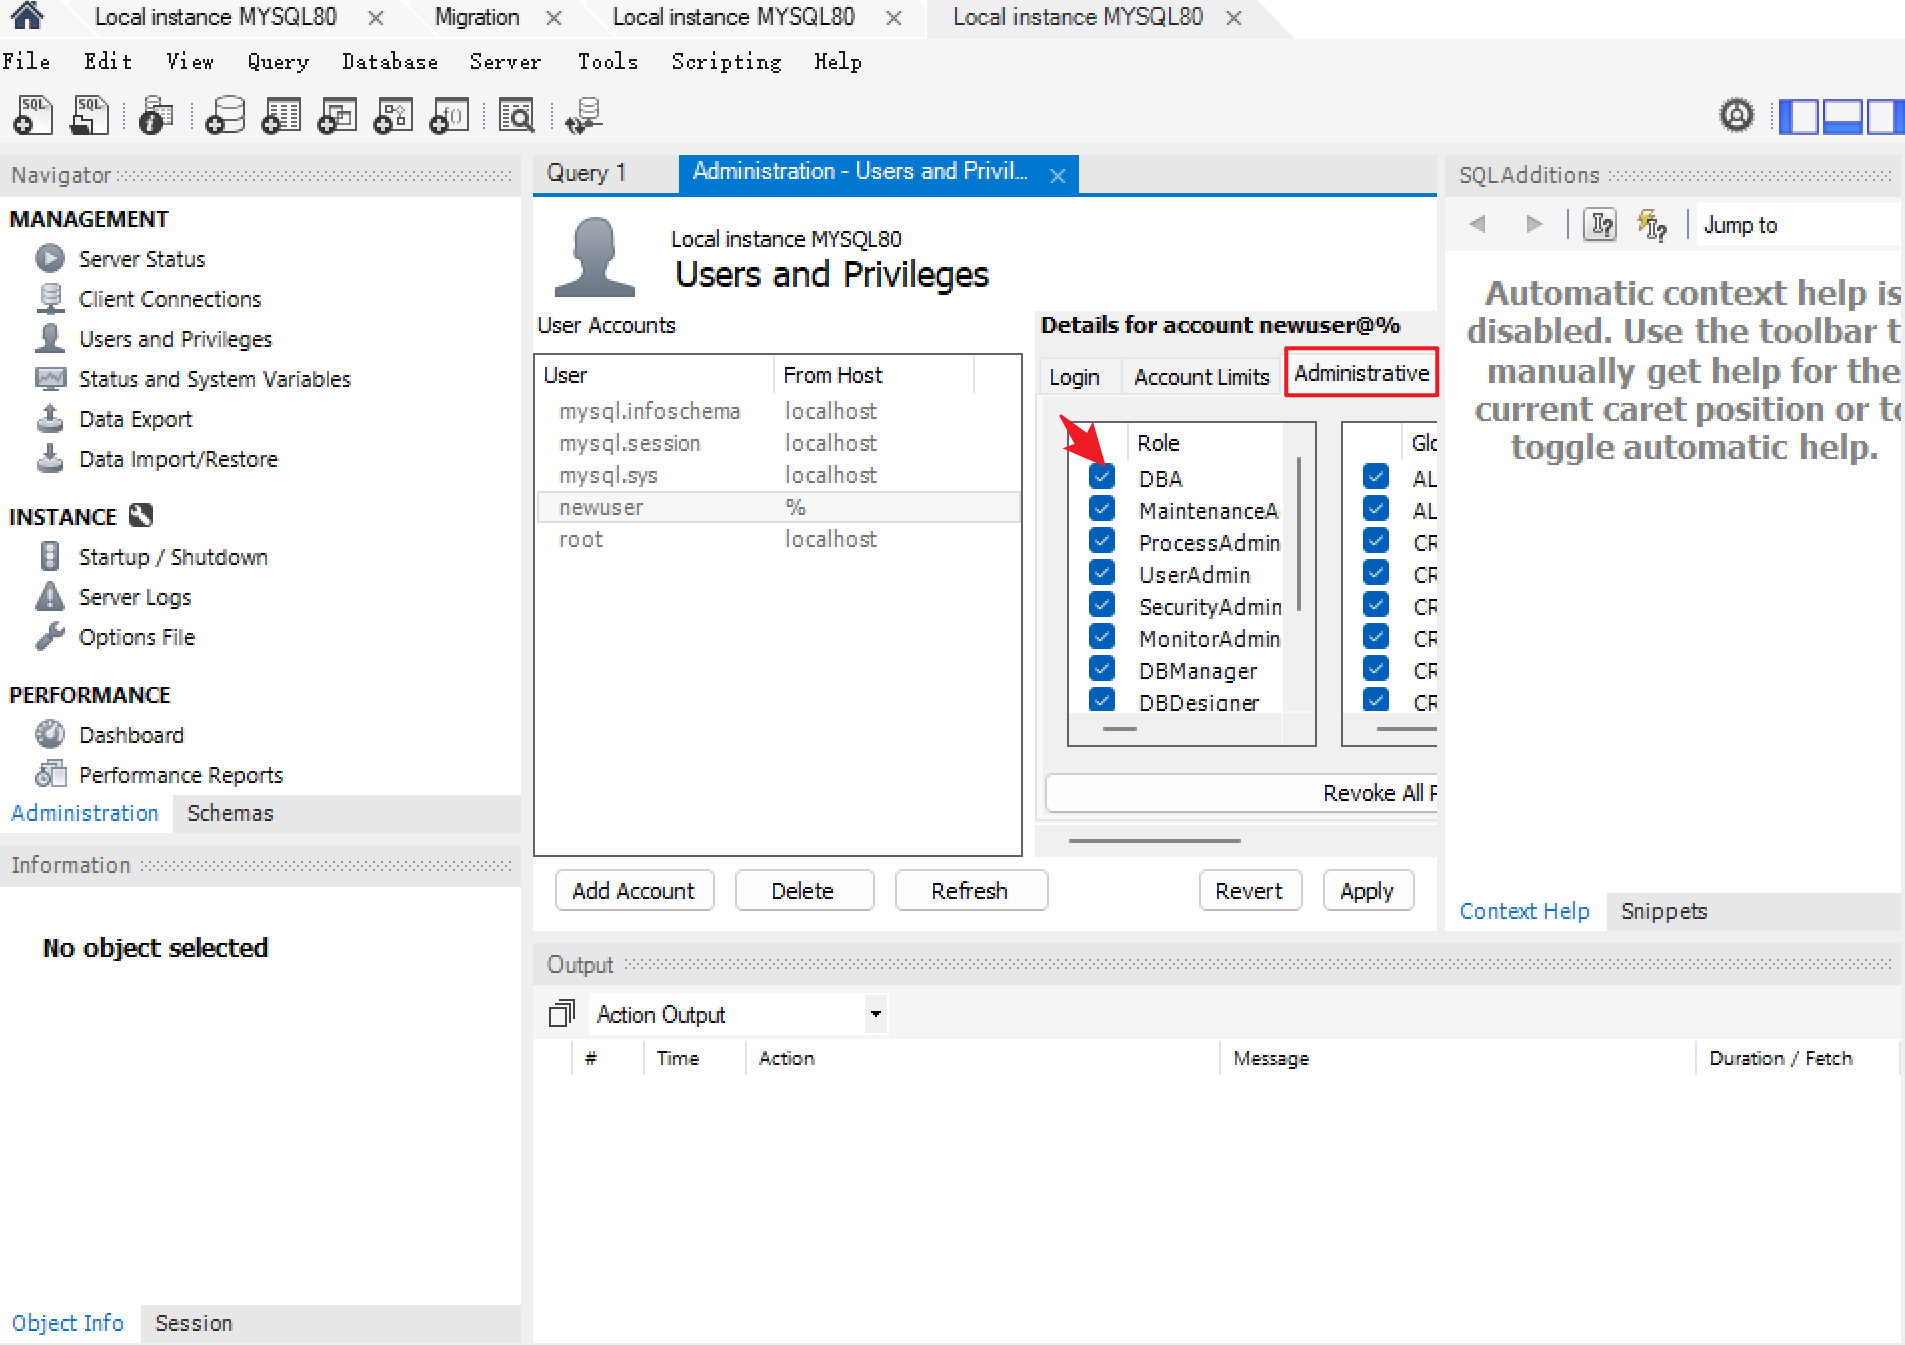
\includegraphics[width=12cm]{../figure/a0000-img004.png} \\
    \footnotesize 图4 数据操作查询截图2
\end{center}
\begin{center}
    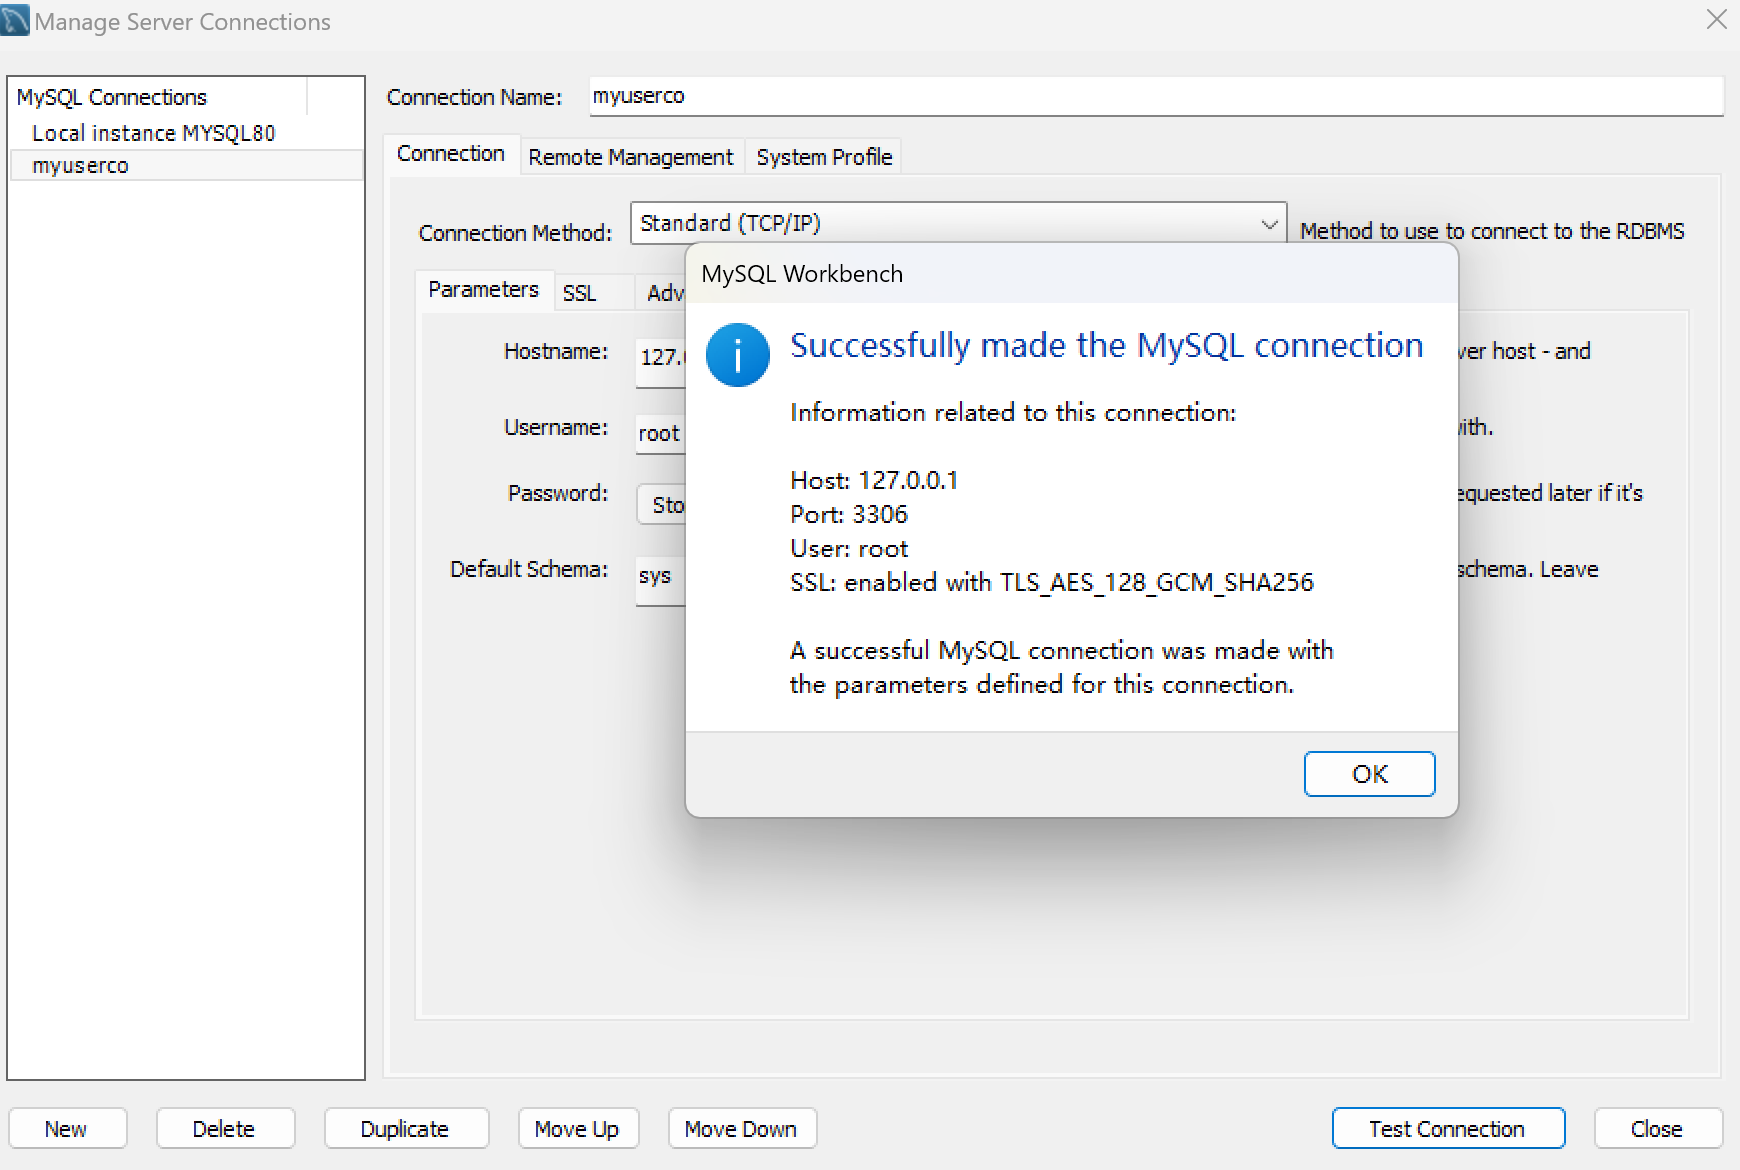
\includegraphics[width=12cm]{../figure/a0000-img005.png} \\
    \footnotesize 图5 数据操作查询截图3
\end{center}
\begin{center}
    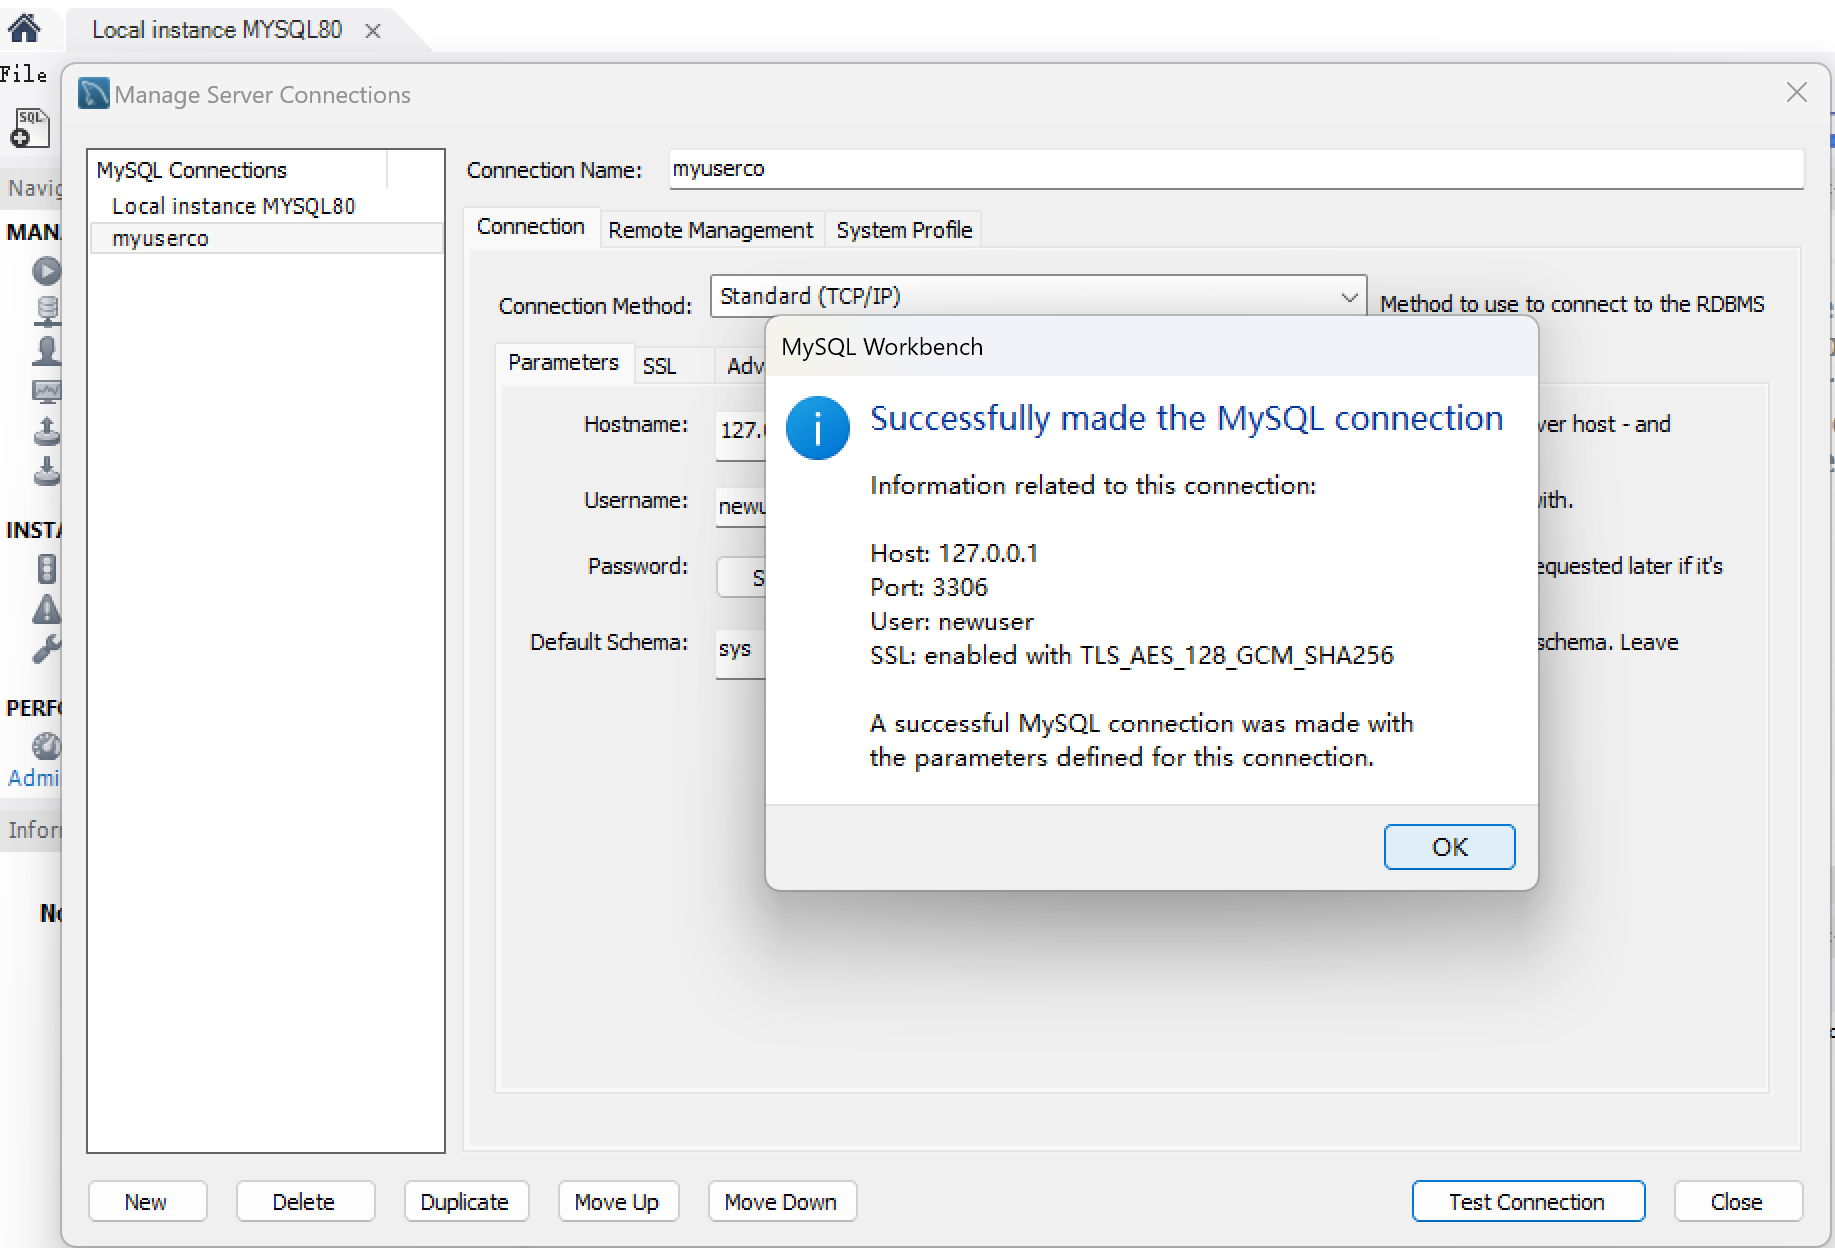
\includegraphics[width=12cm]{../figure/a0000-img006.png} \\
    \footnotesize 图6 数据操作查询截图4
\end{center}
\begin{center}
    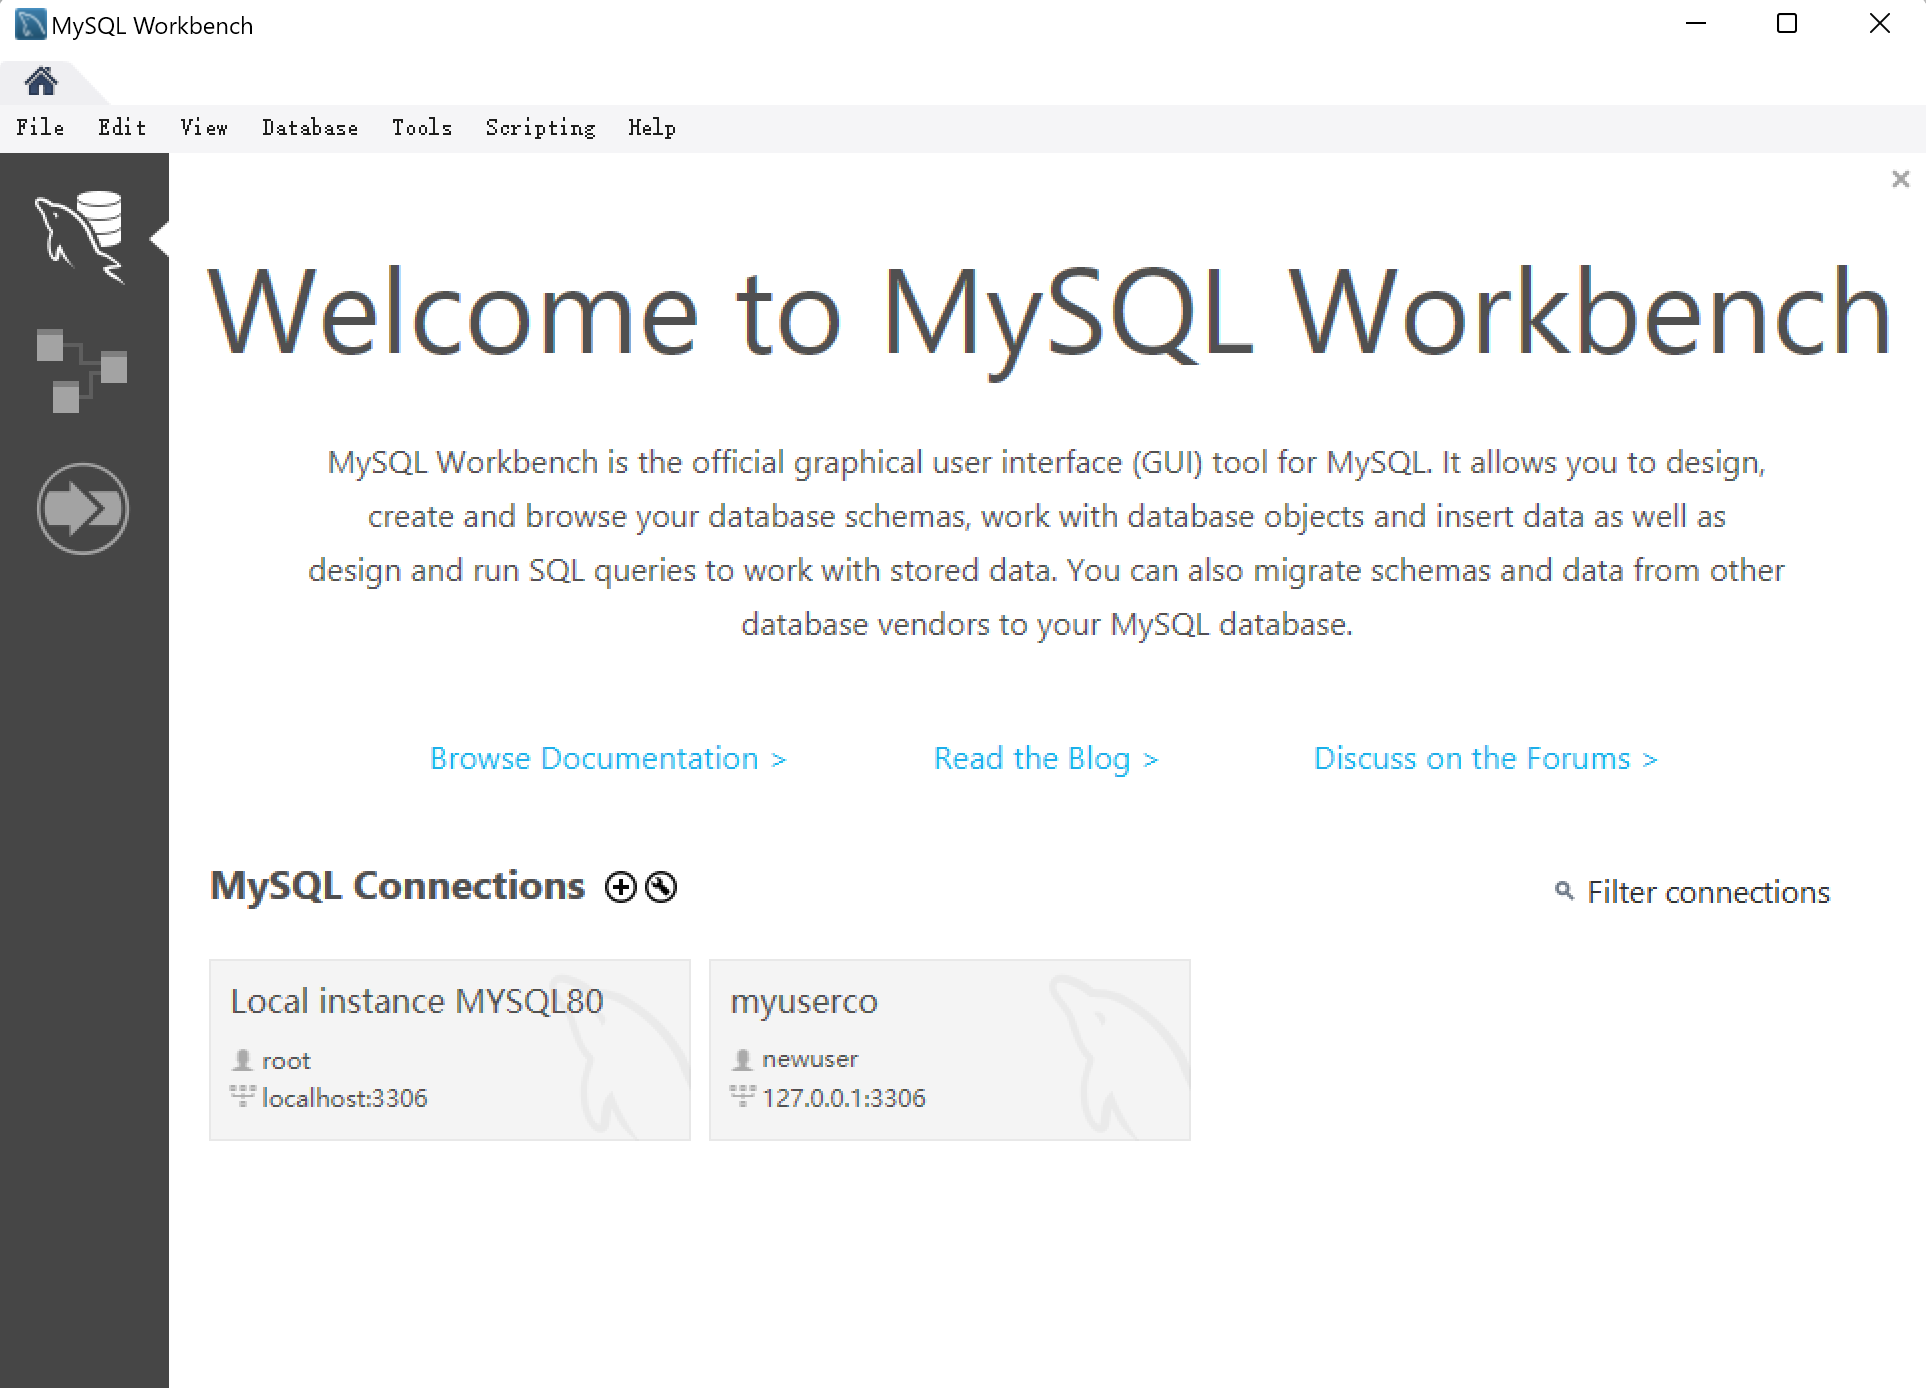
\includegraphics[width=12cm]{../figure/a0000-img007.png} \\
    \footnotesize 图7 数据操作查询截图5
\end{center}
\begin{center}
    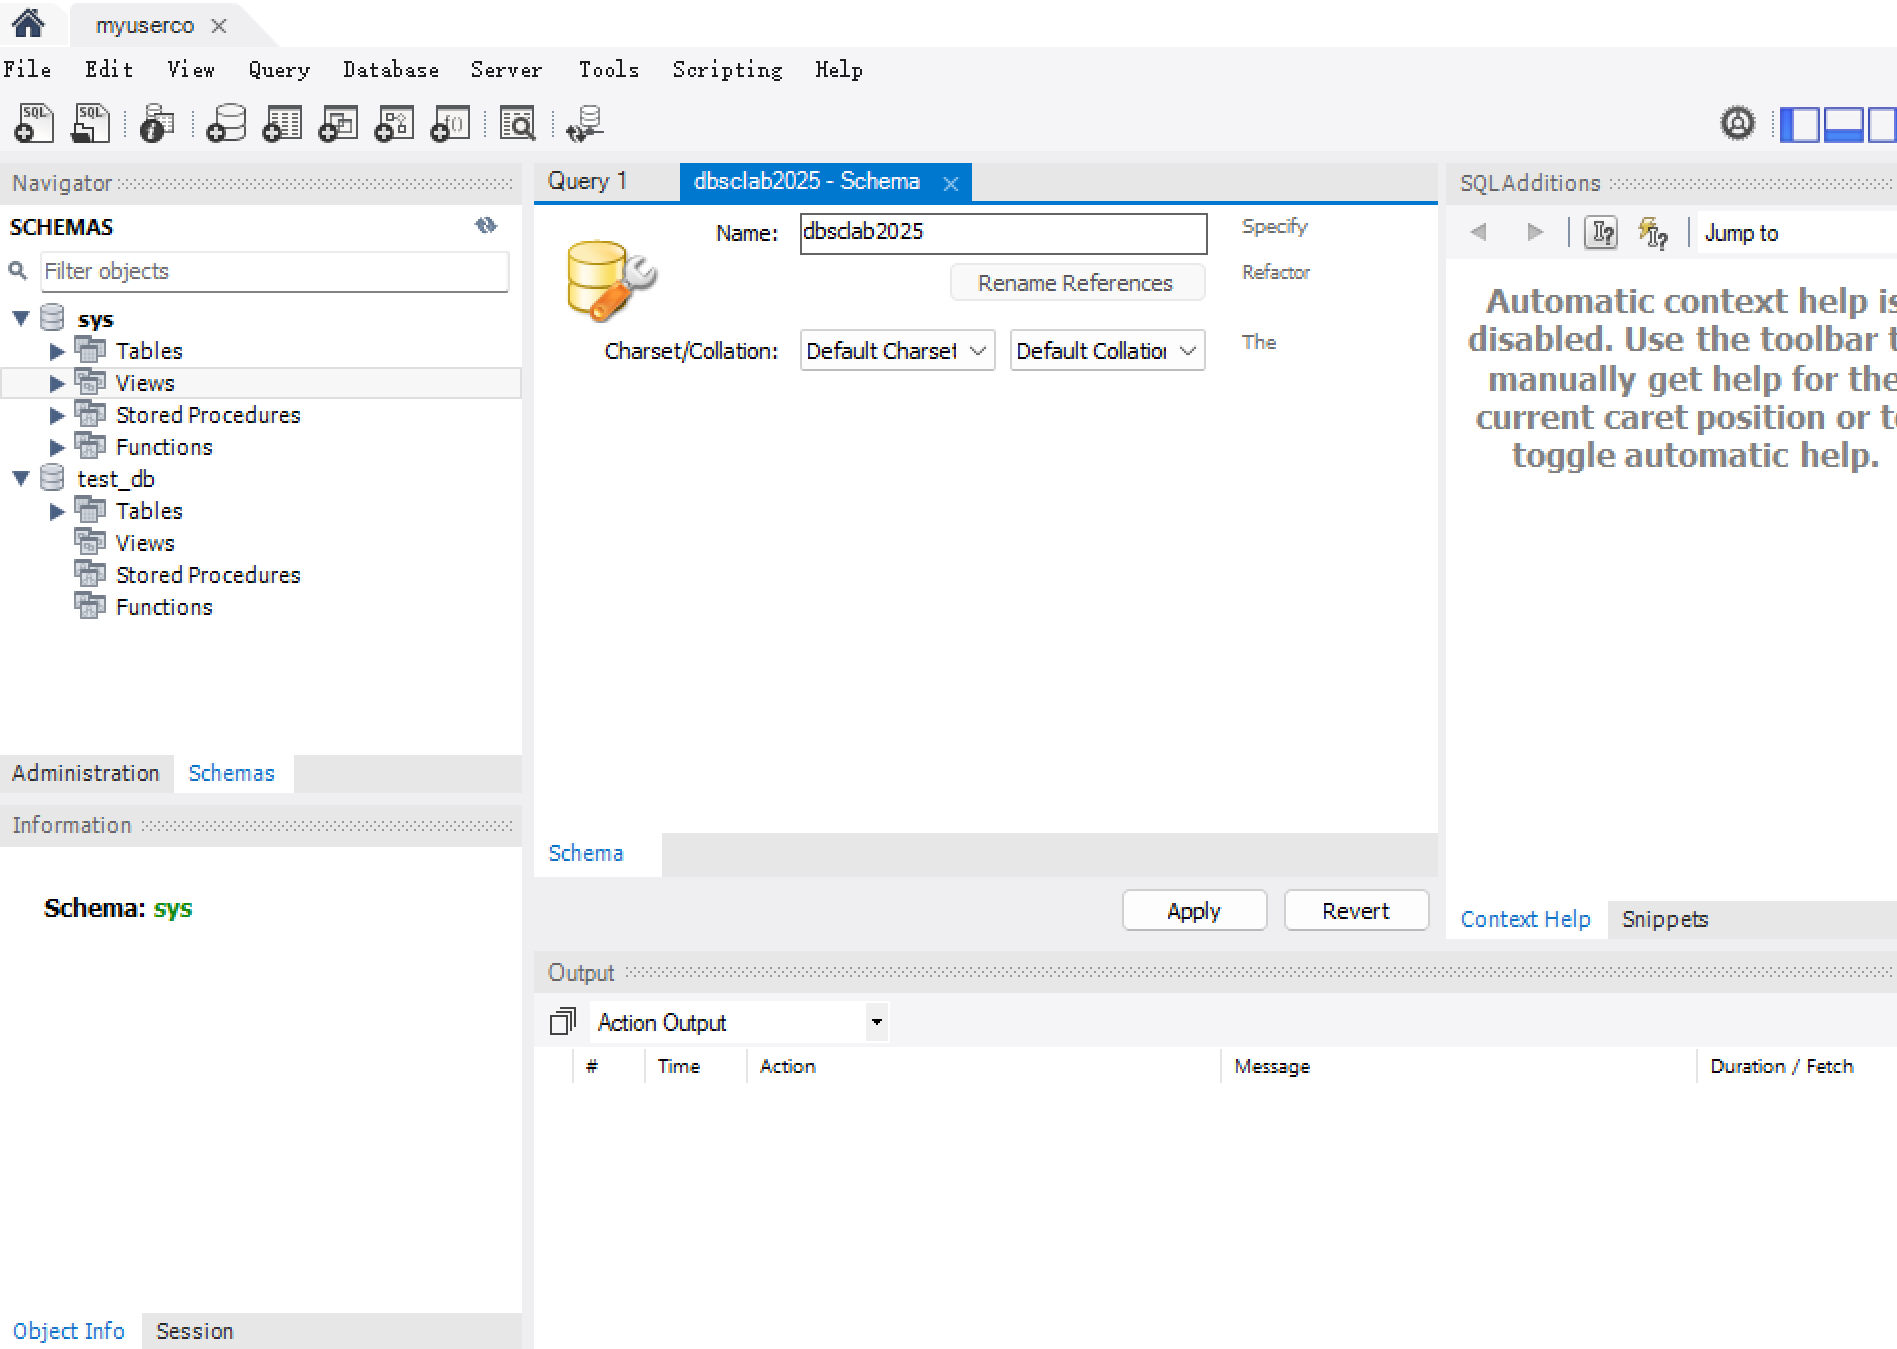
\includegraphics[width=12cm]{../figure/a0000-img008.png} \\
    \footnotesize 图8 数据操作查询截图6
\end{center}
\begin{center}
    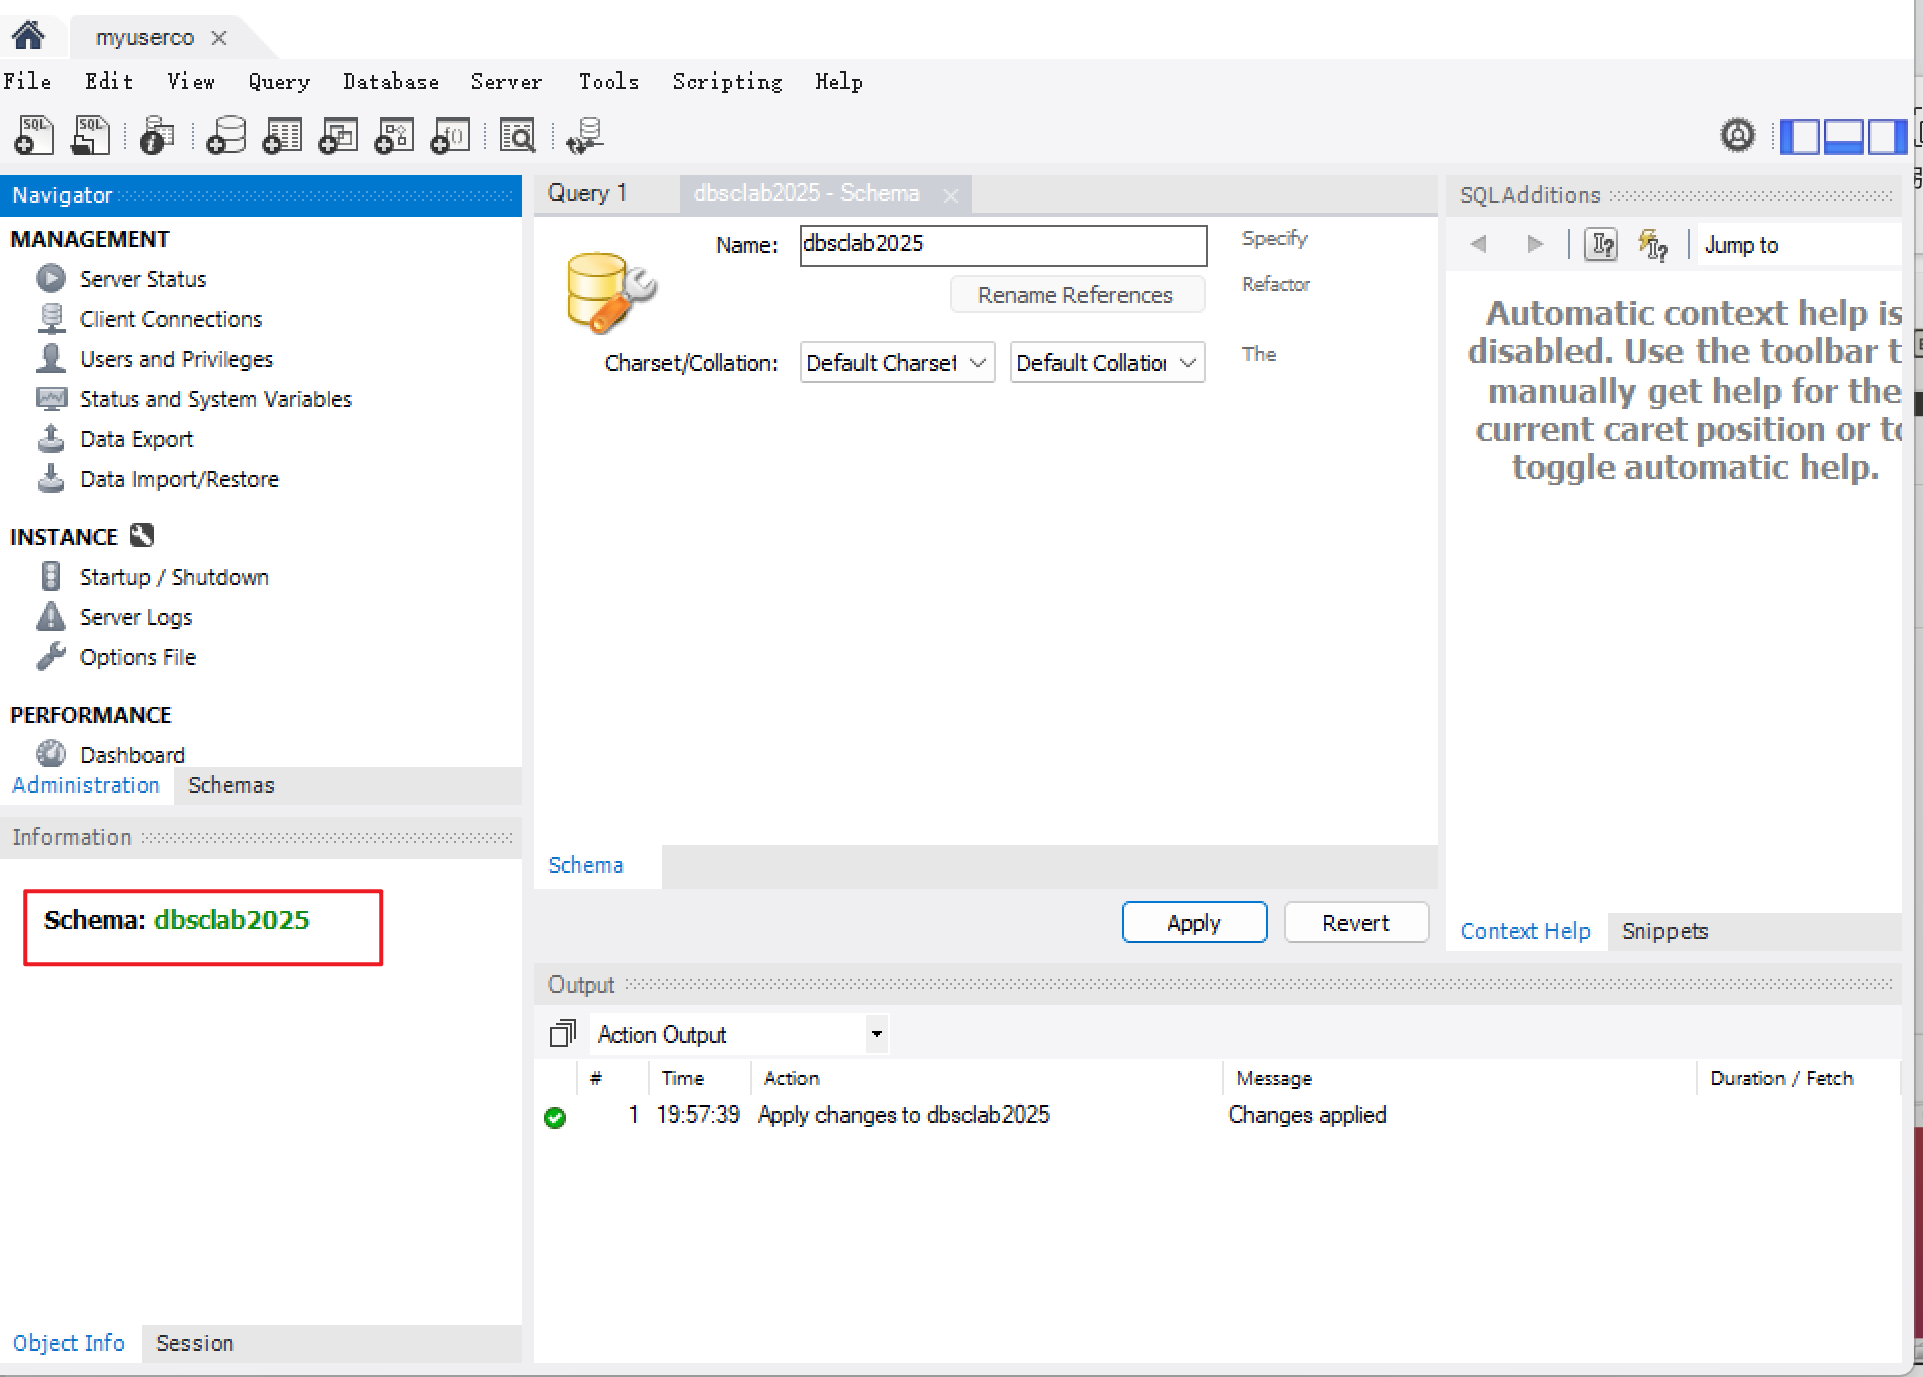
\includegraphics[width=12cm]{../figure/a0000-img009.png} \\
    \footnotesize 图9 数据操作查询截图7
\end{center}
\begin{center}
    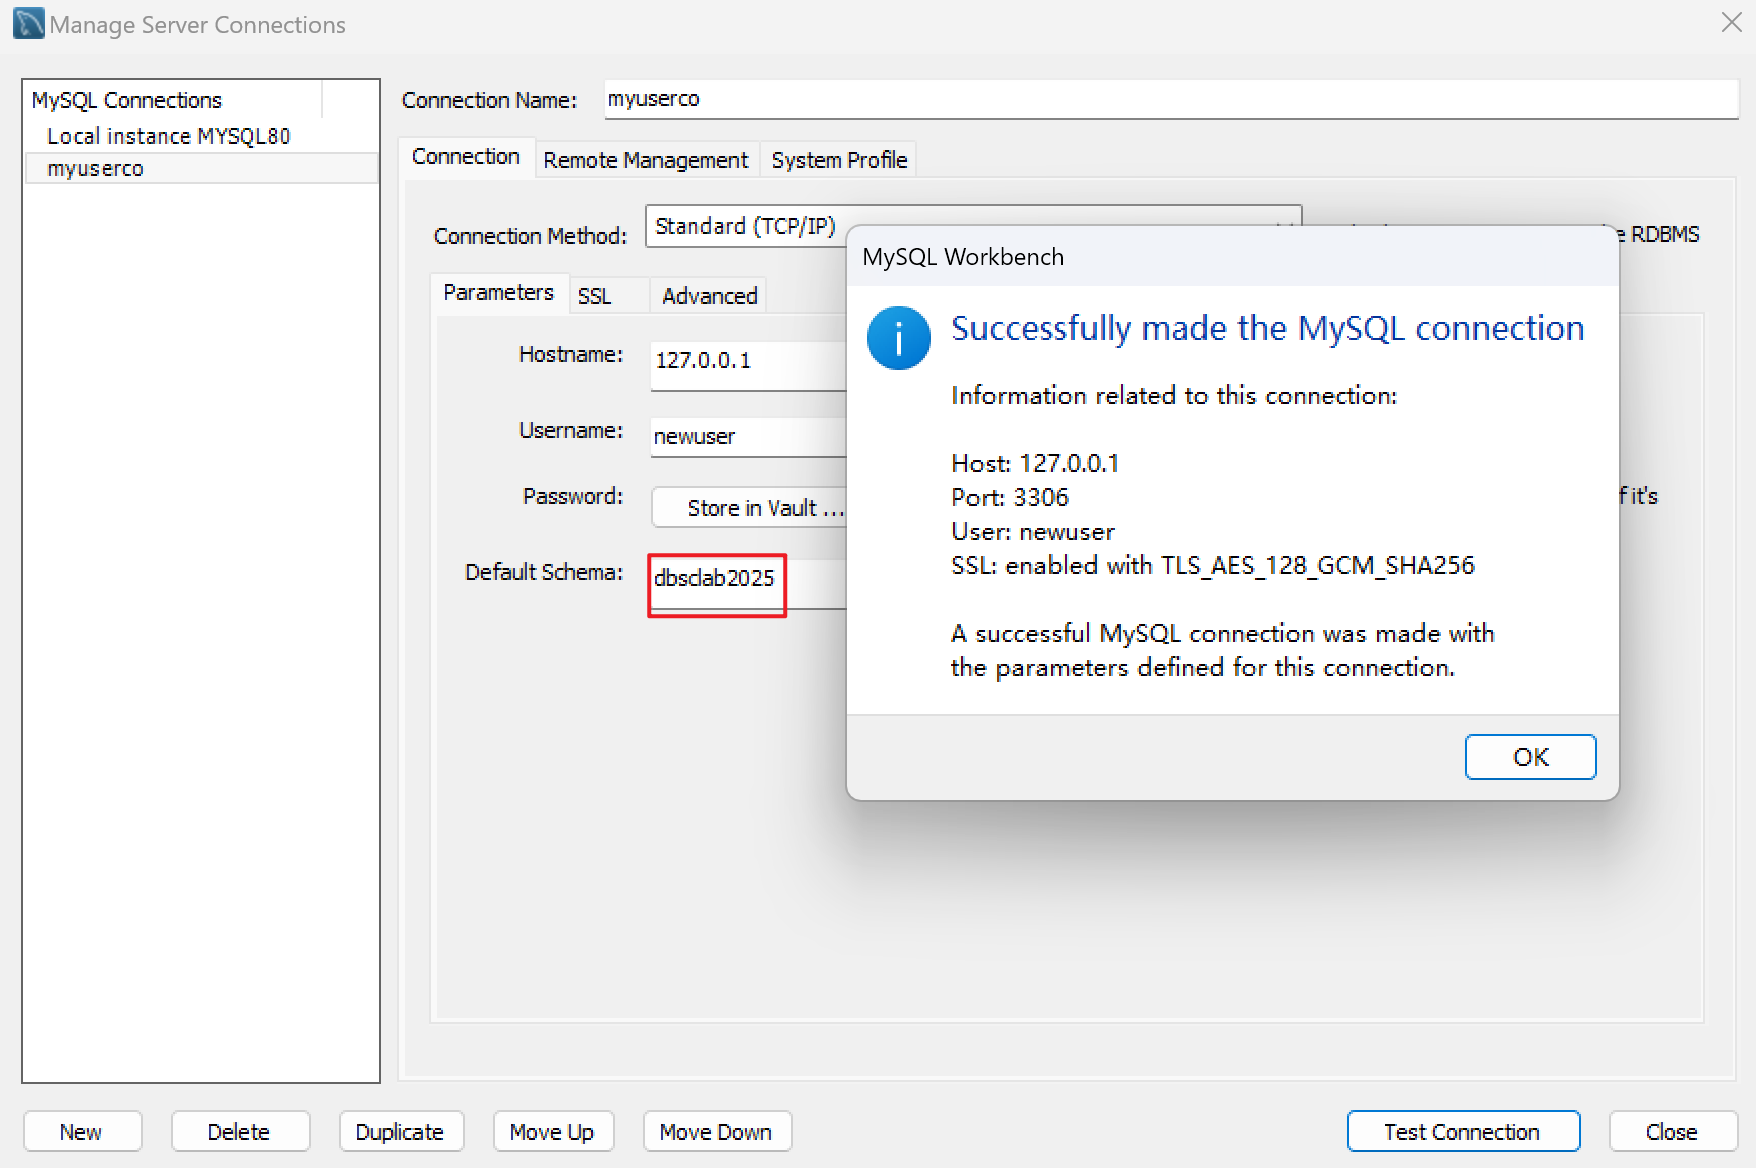
\includegraphics[width=12cm]{../figure/a0000-img010.png} \\
    \footnotesize 图10 数据操作查询截图8
\end{center}
\begin{center}
    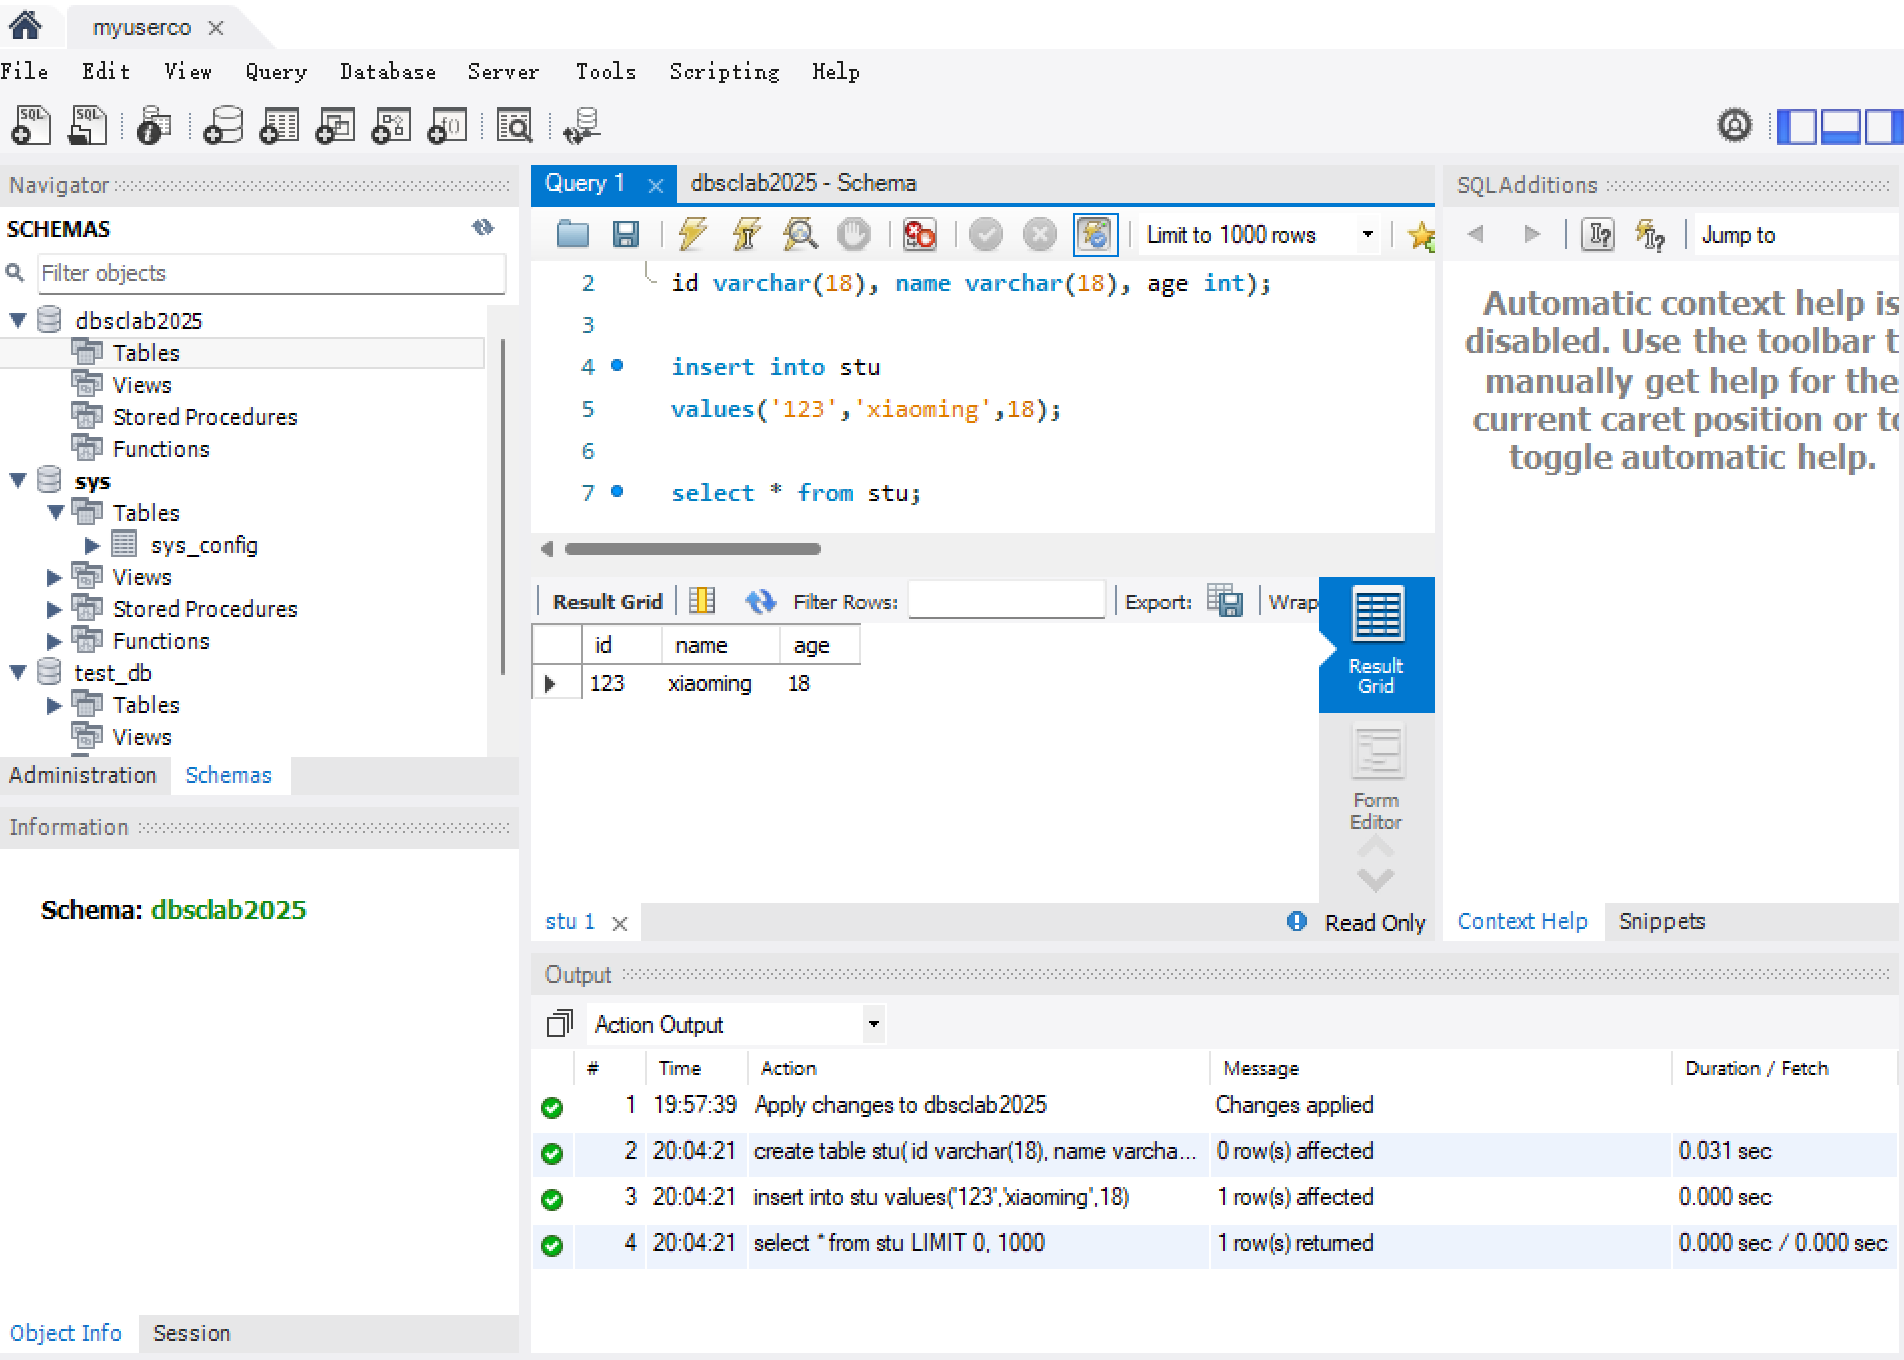
\includegraphics[width=12cm]{../figure/a0000-img011.png} \\
    \footnotesize 图11 数据操作查询截图9
\end{center}
\begin{center}
    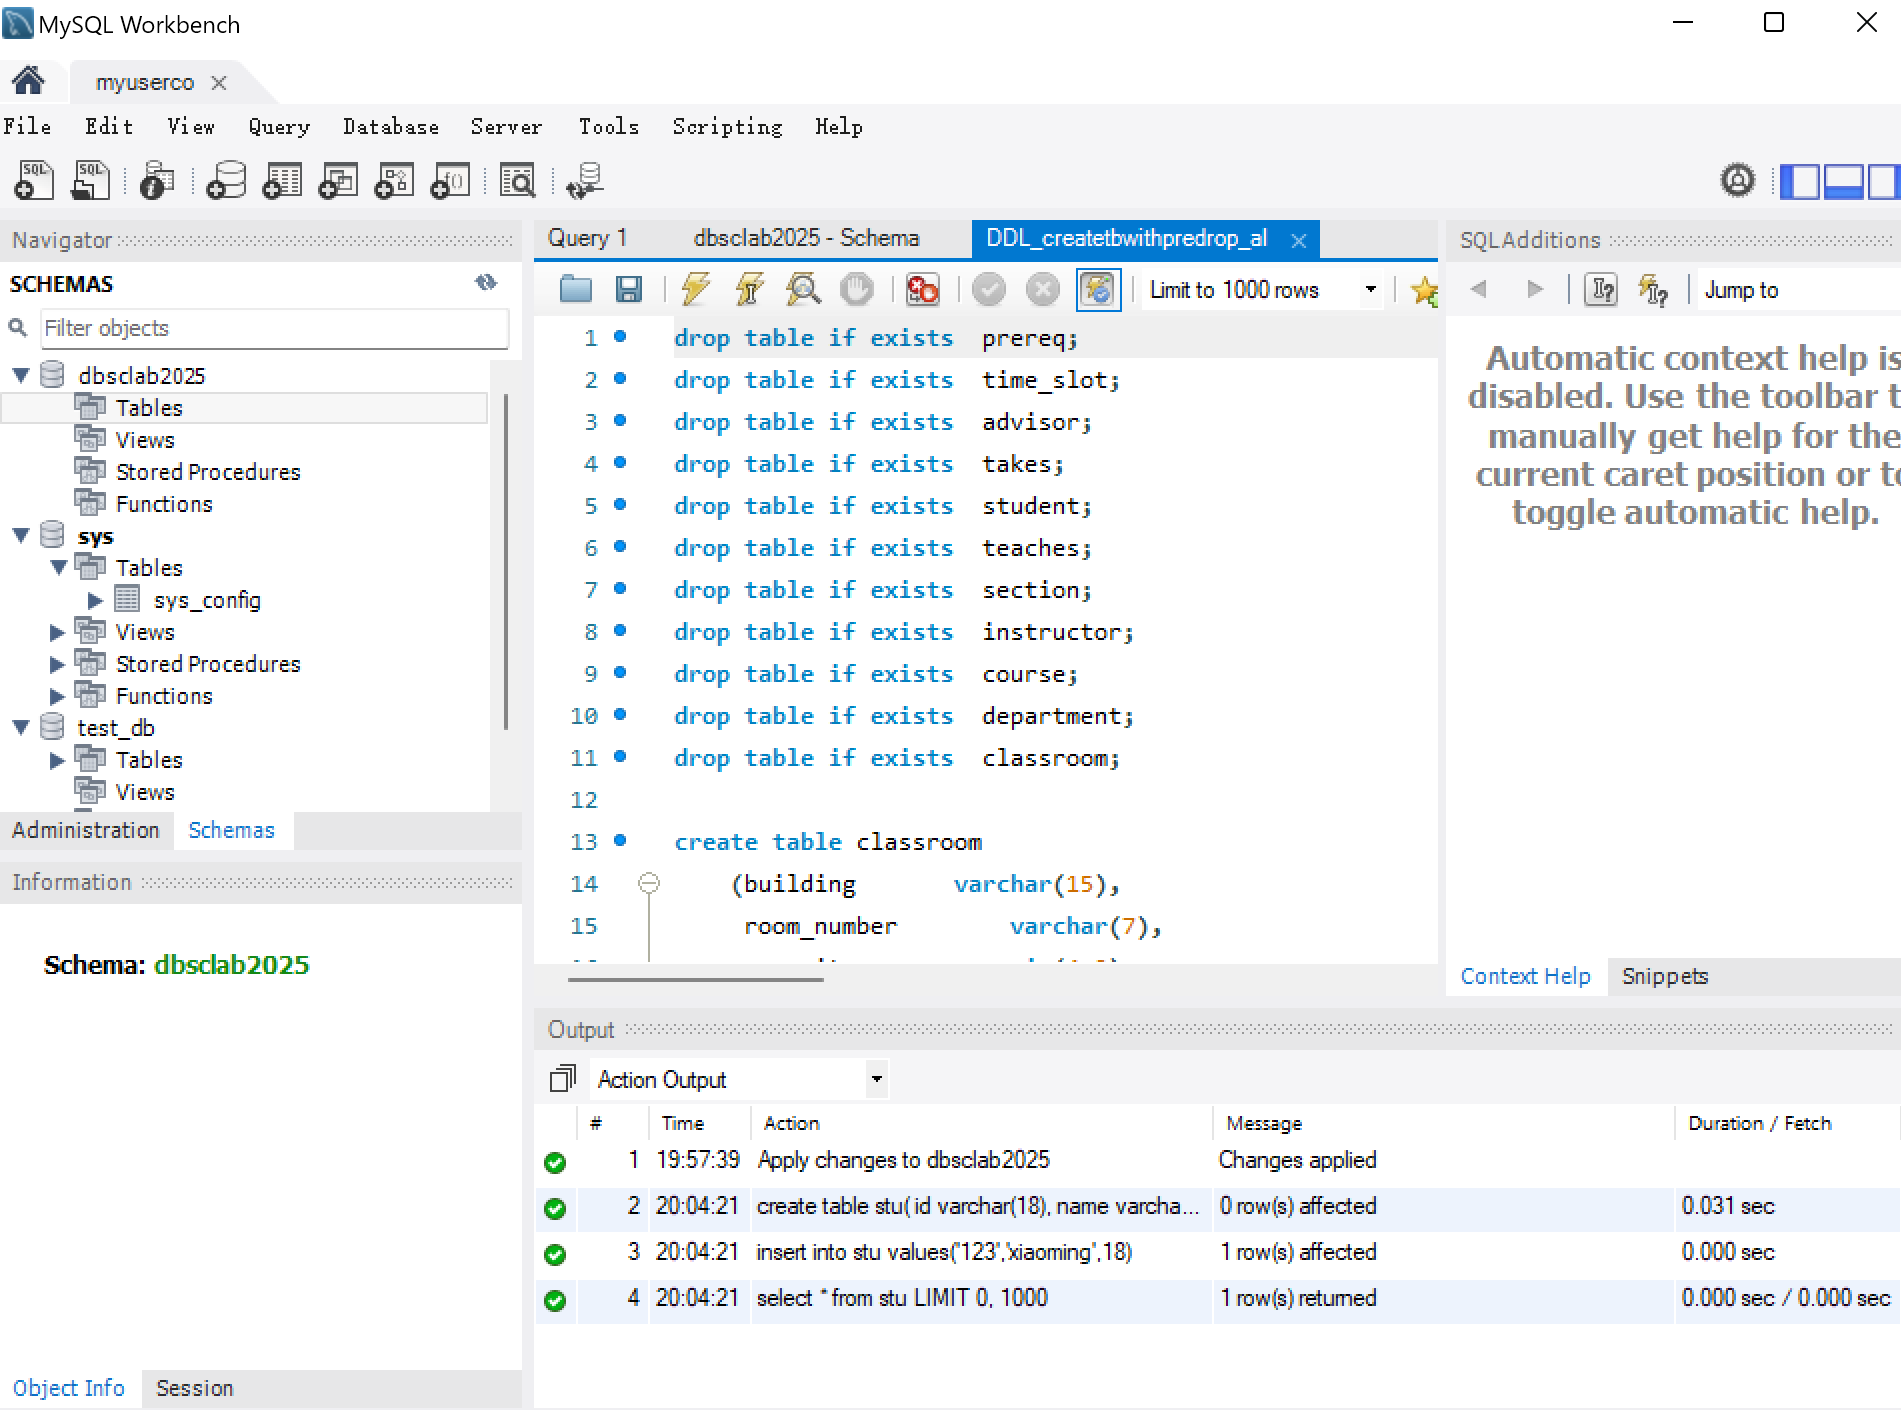
\includegraphics[width=12cm]{../figure/a0000-img012.png} \\
    \footnotesize 图12 数据操作查询截图10
\end{center}
\begin{center}
    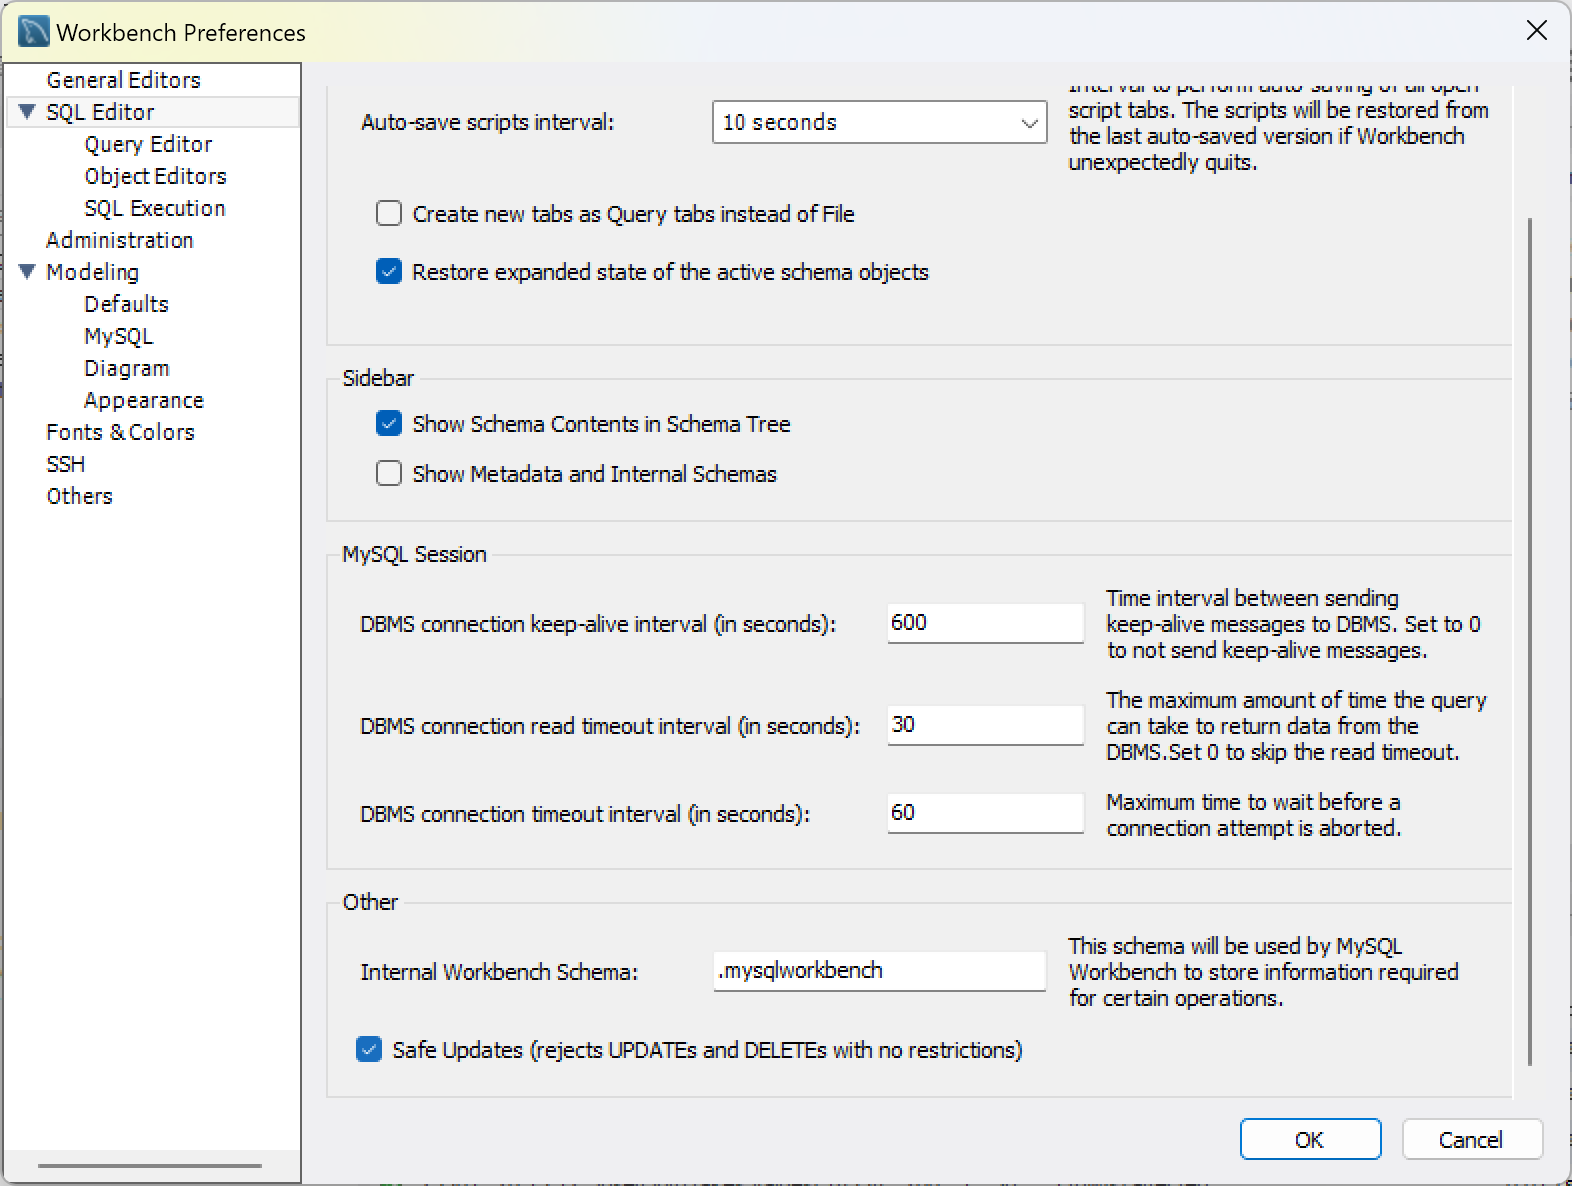
\includegraphics[width=12cm]{../figure/a0000-img013.png} \\
    \footnotesize 图13 数据操作查询截图11
\end{center}
\begin{center}
    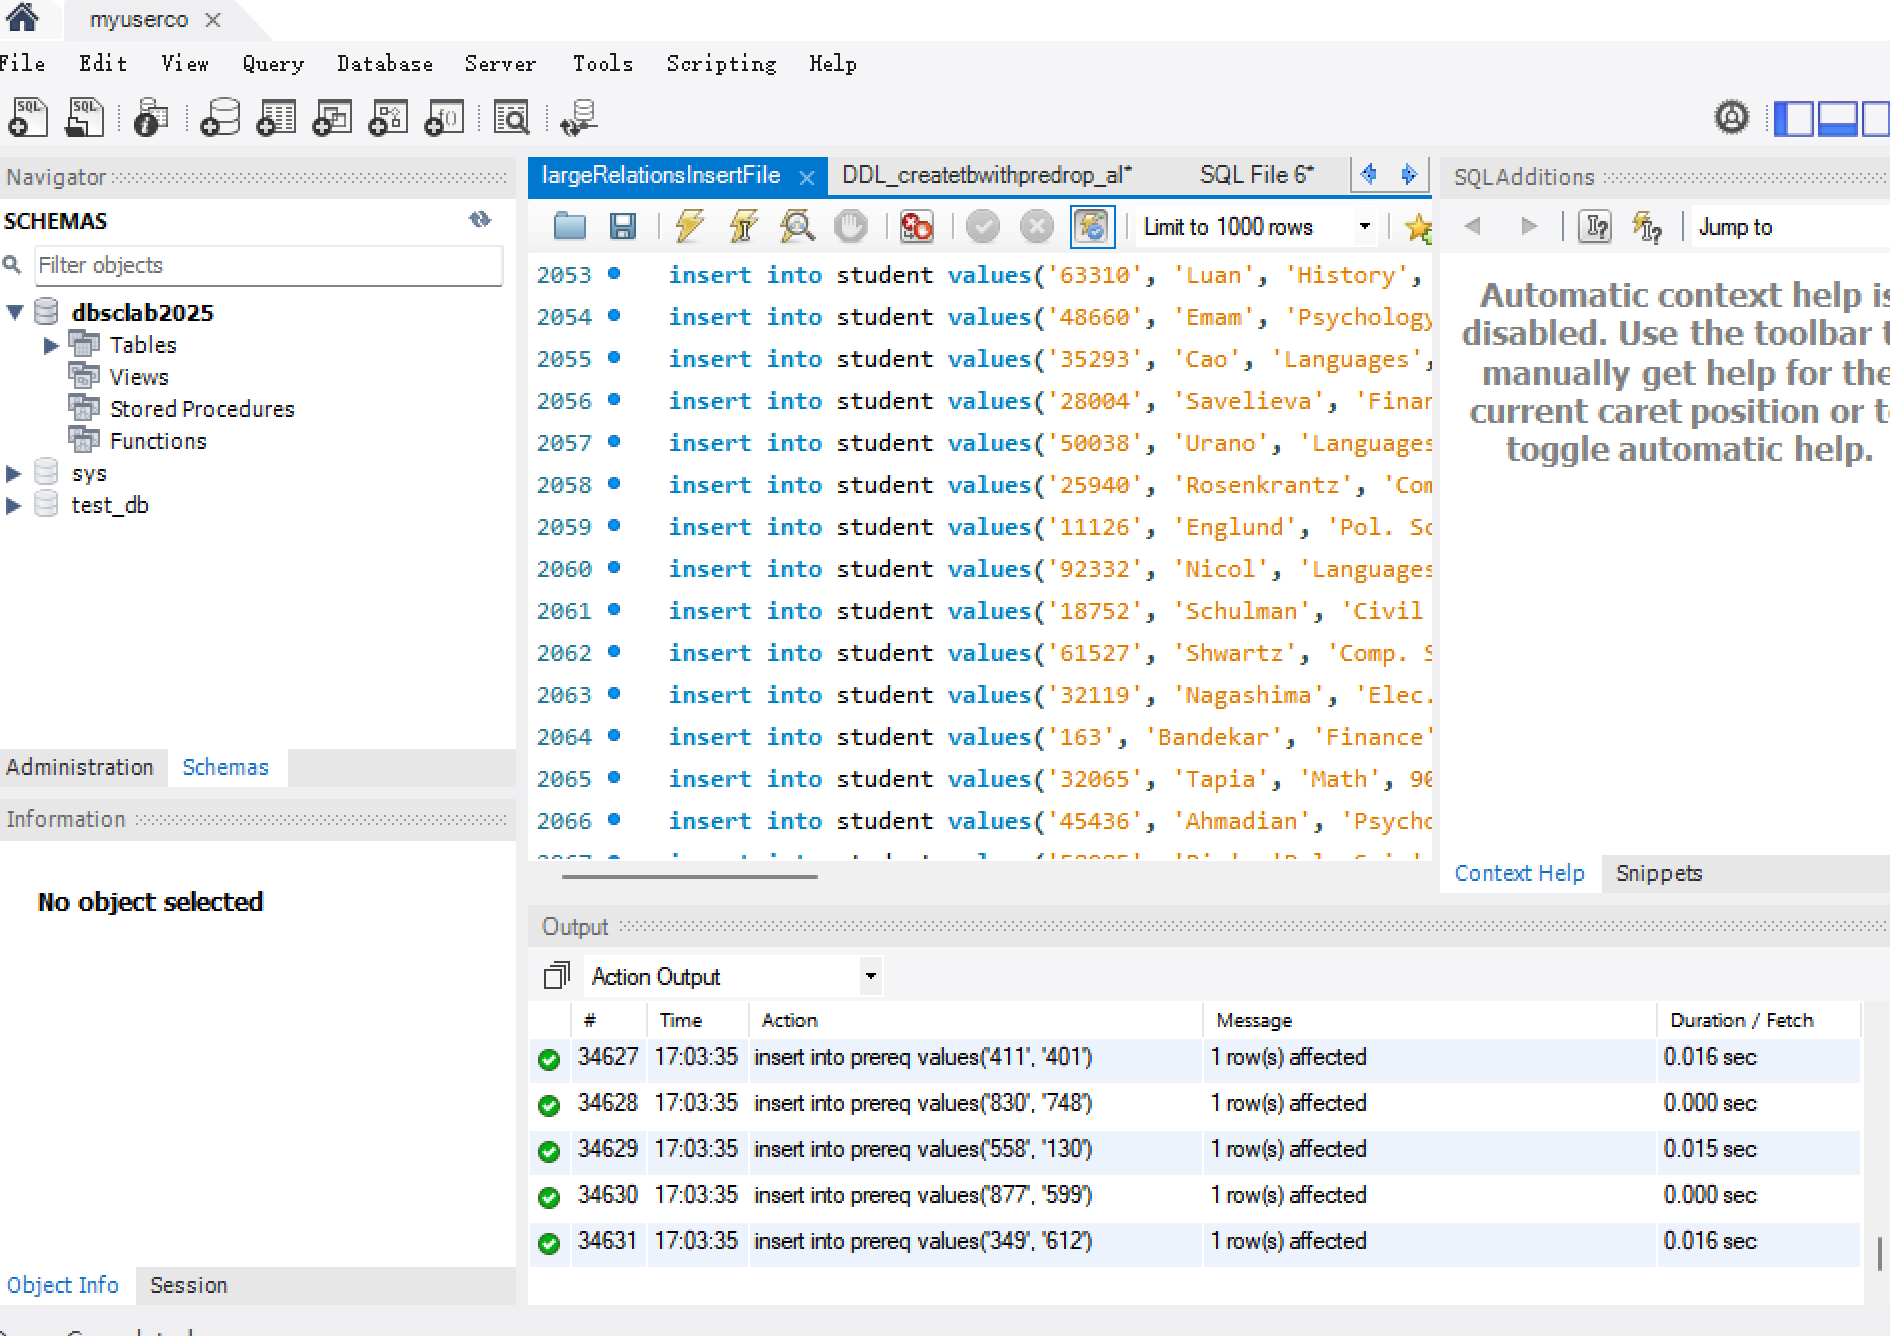
\includegraphics[width=12cm]{../figure/a0000-img014.png} \\
    \footnotesize 图14 数据操作查询截图12
\end{center}
\begin{center}
    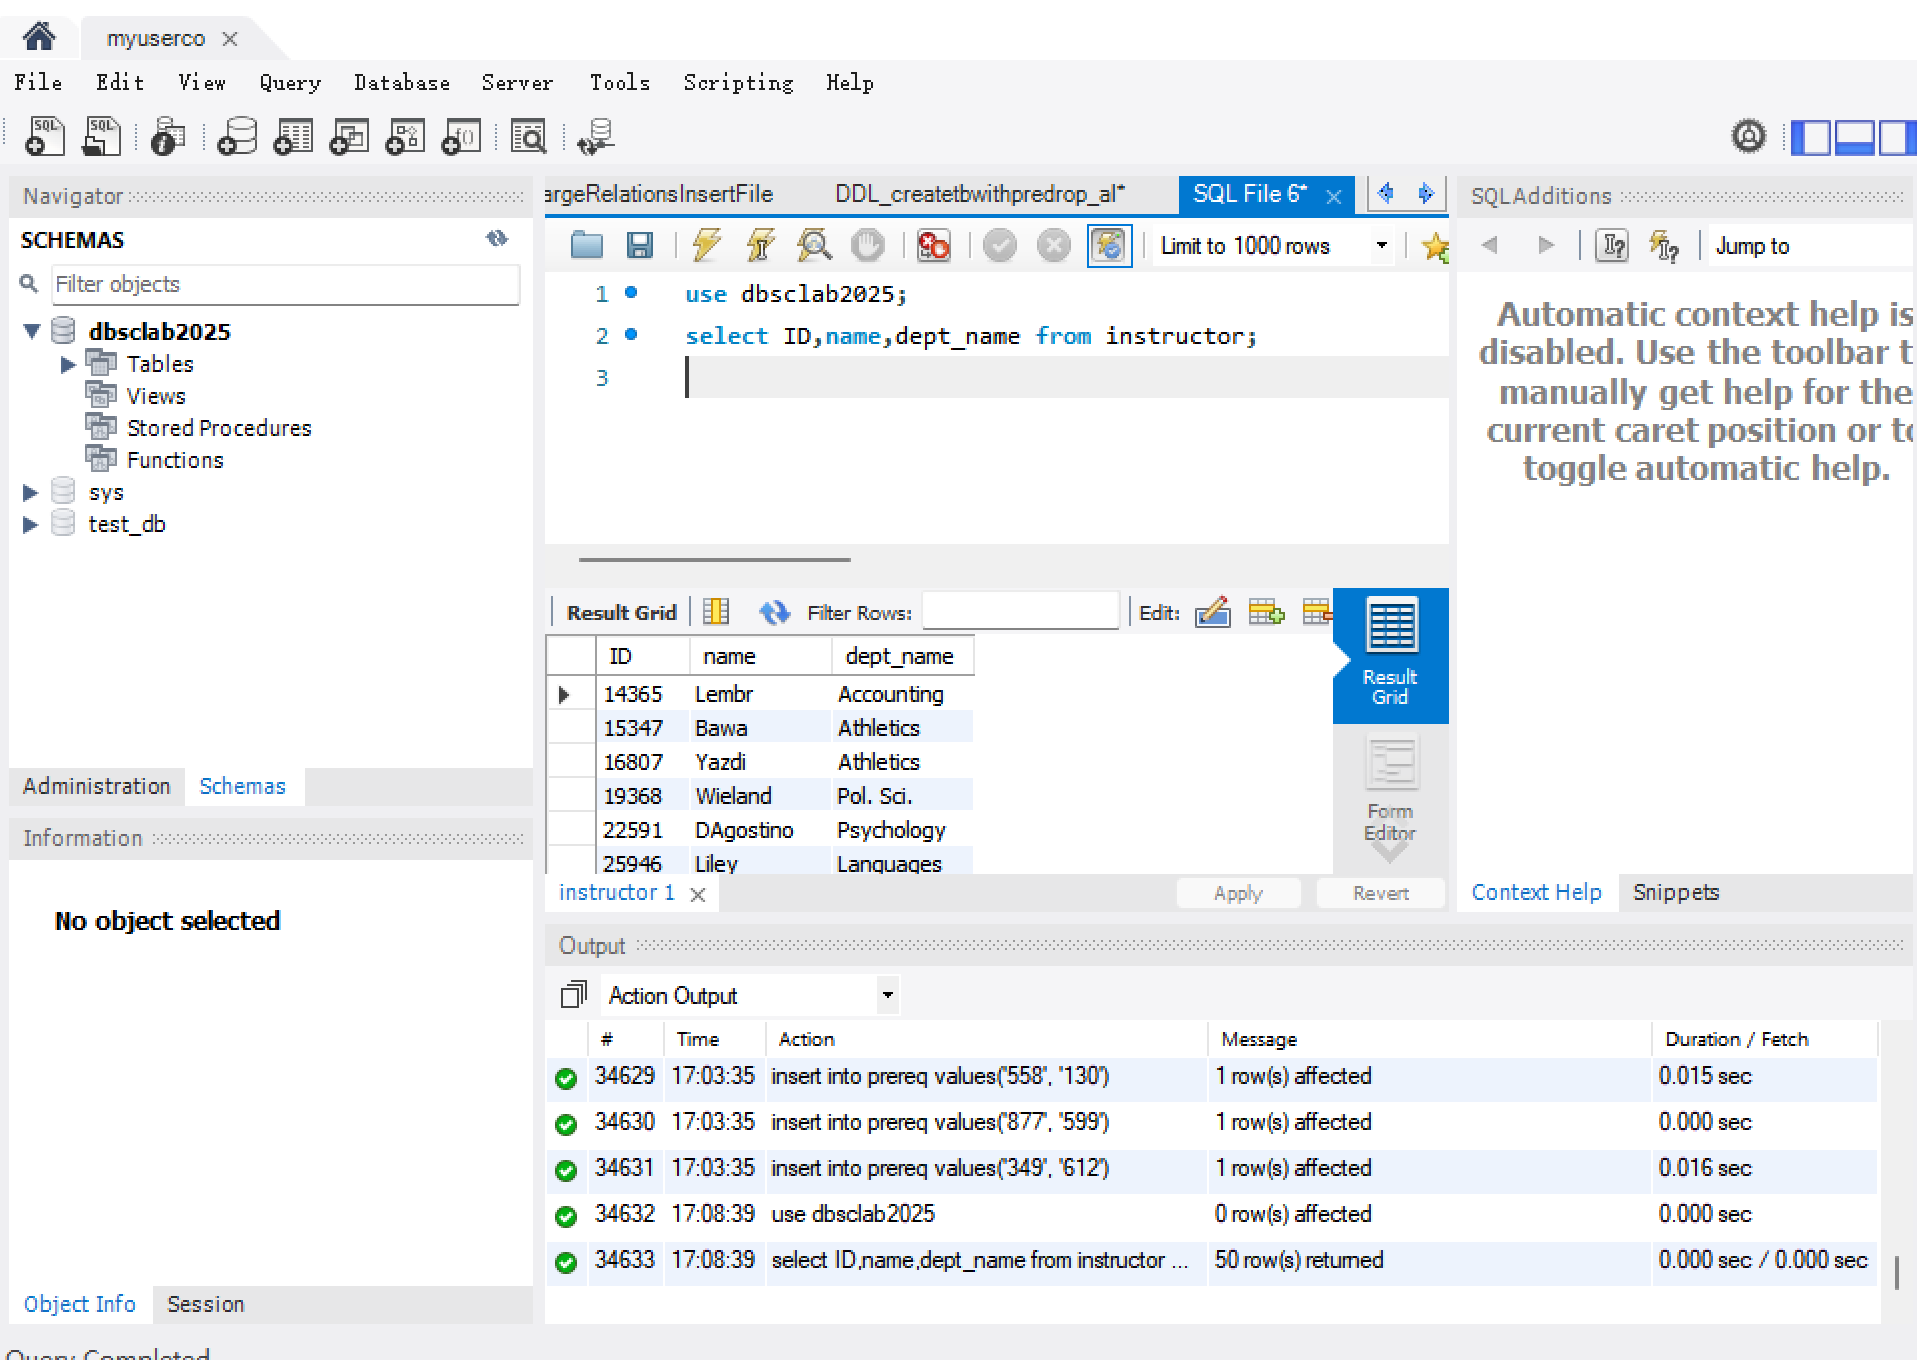
\includegraphics[width=12cm]{../figure/a0000-img015.png} \\
    \footnotesize 图15 数据操作查询截图13
\end{center}
\begin{center}
    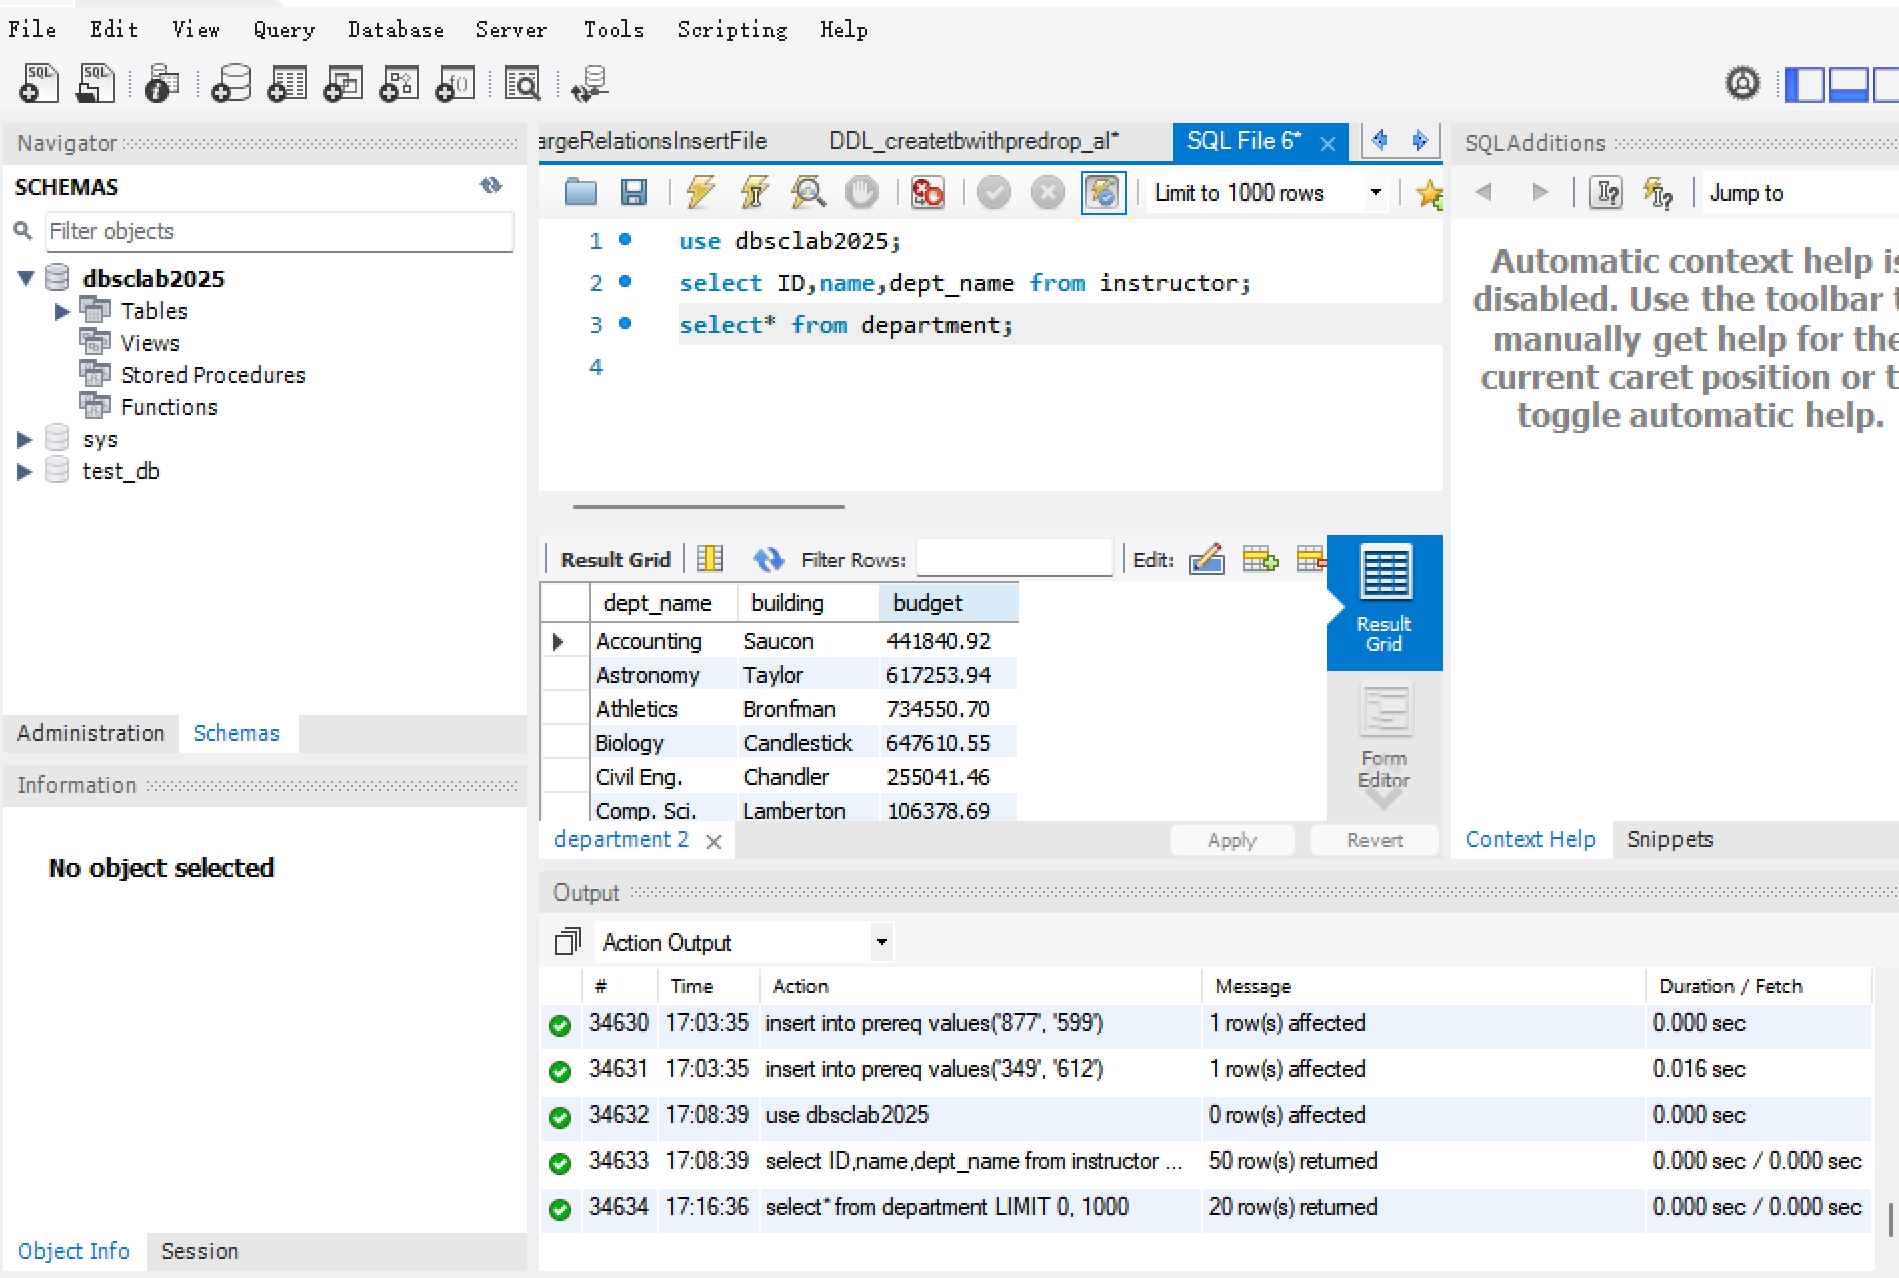
\includegraphics[width=12cm]{../figure/a0000-img016.png} \\
    \footnotesize 图16 数据操作查询截图14
\end{center}
\begin{center}
    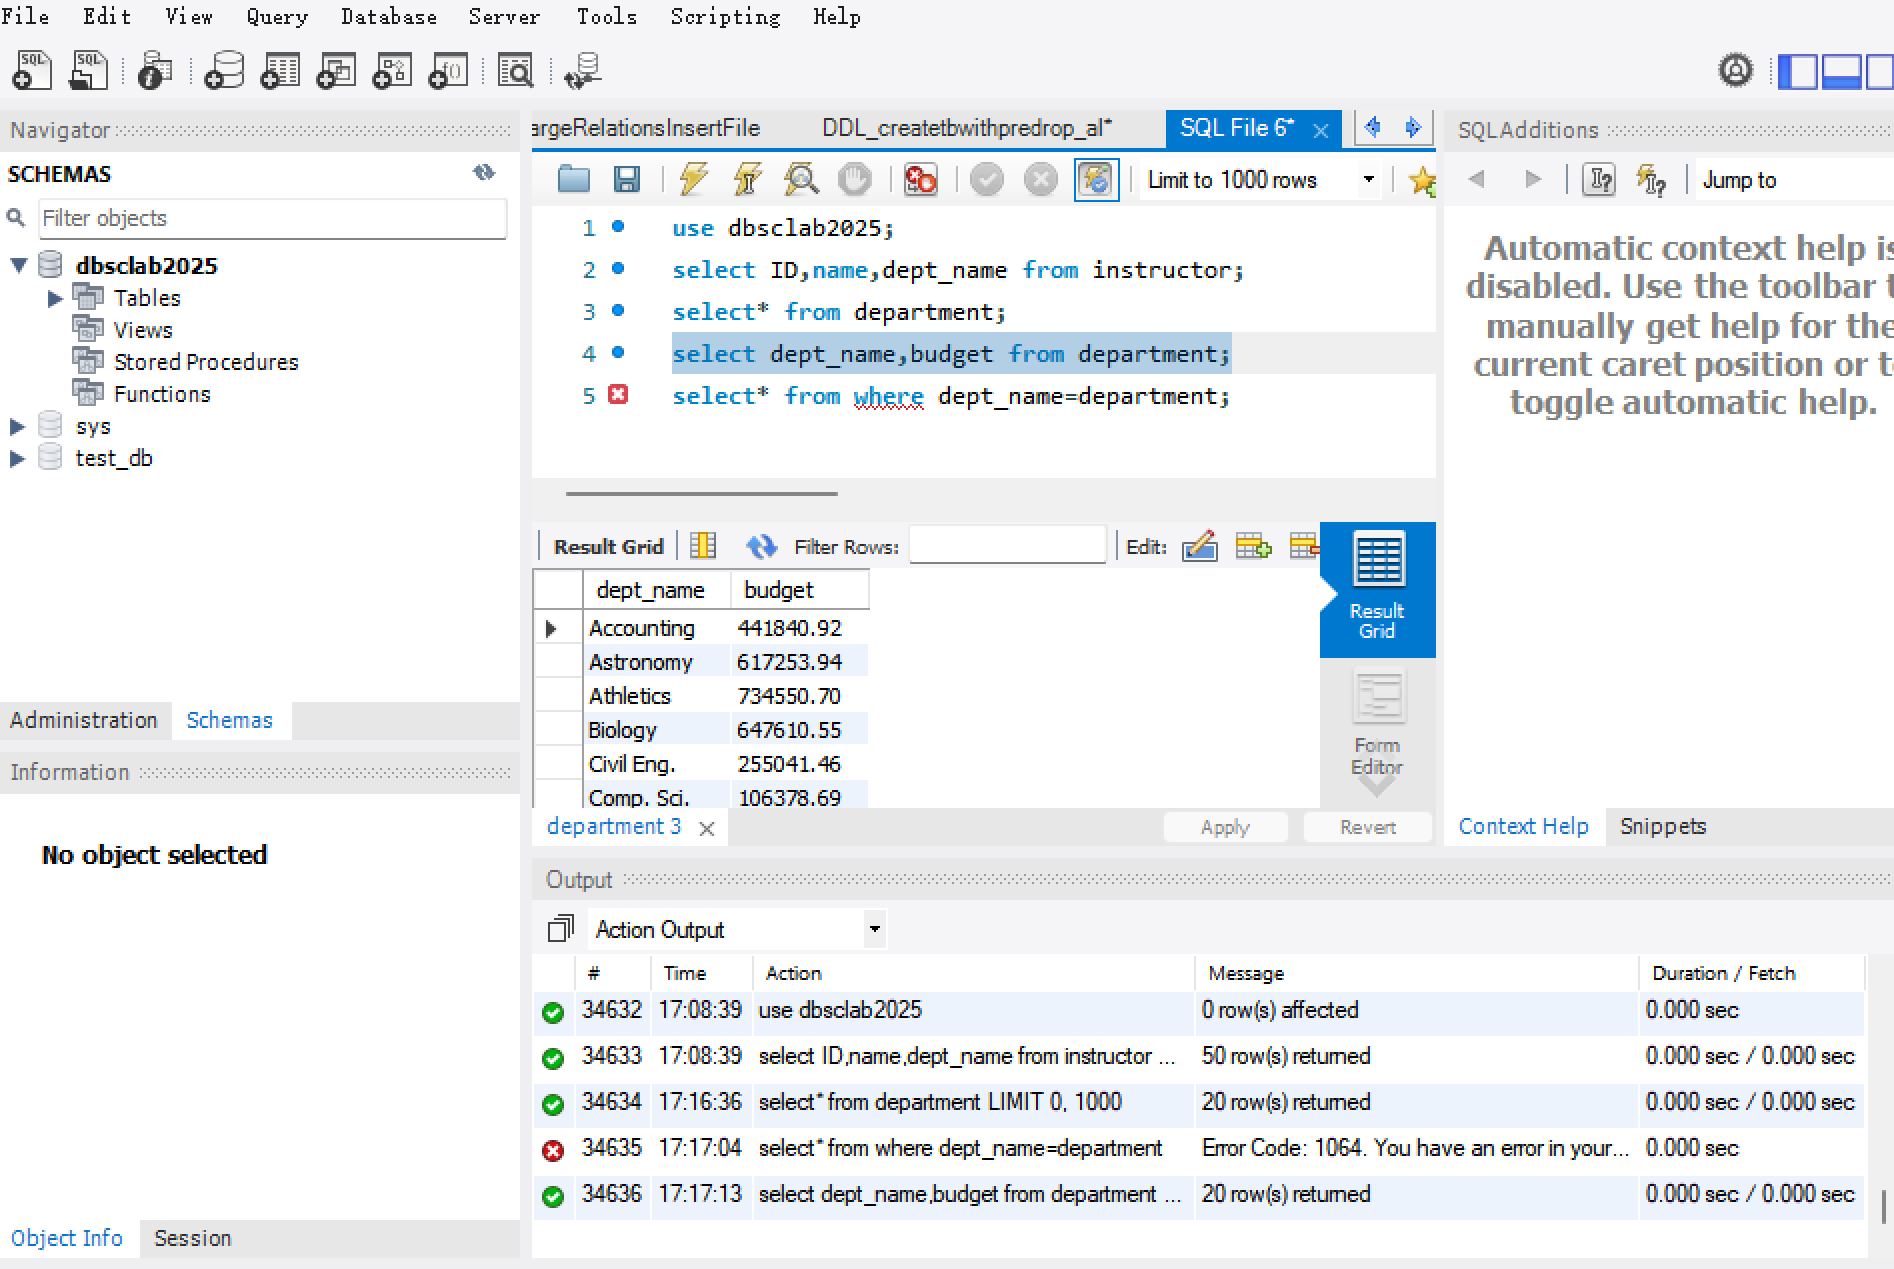
\includegraphics[width=12cm]{../figure/a0000-img017.png} \\
    \footnotesize 图17 数据操作查询截图15
\end{center}
\begin{center}
    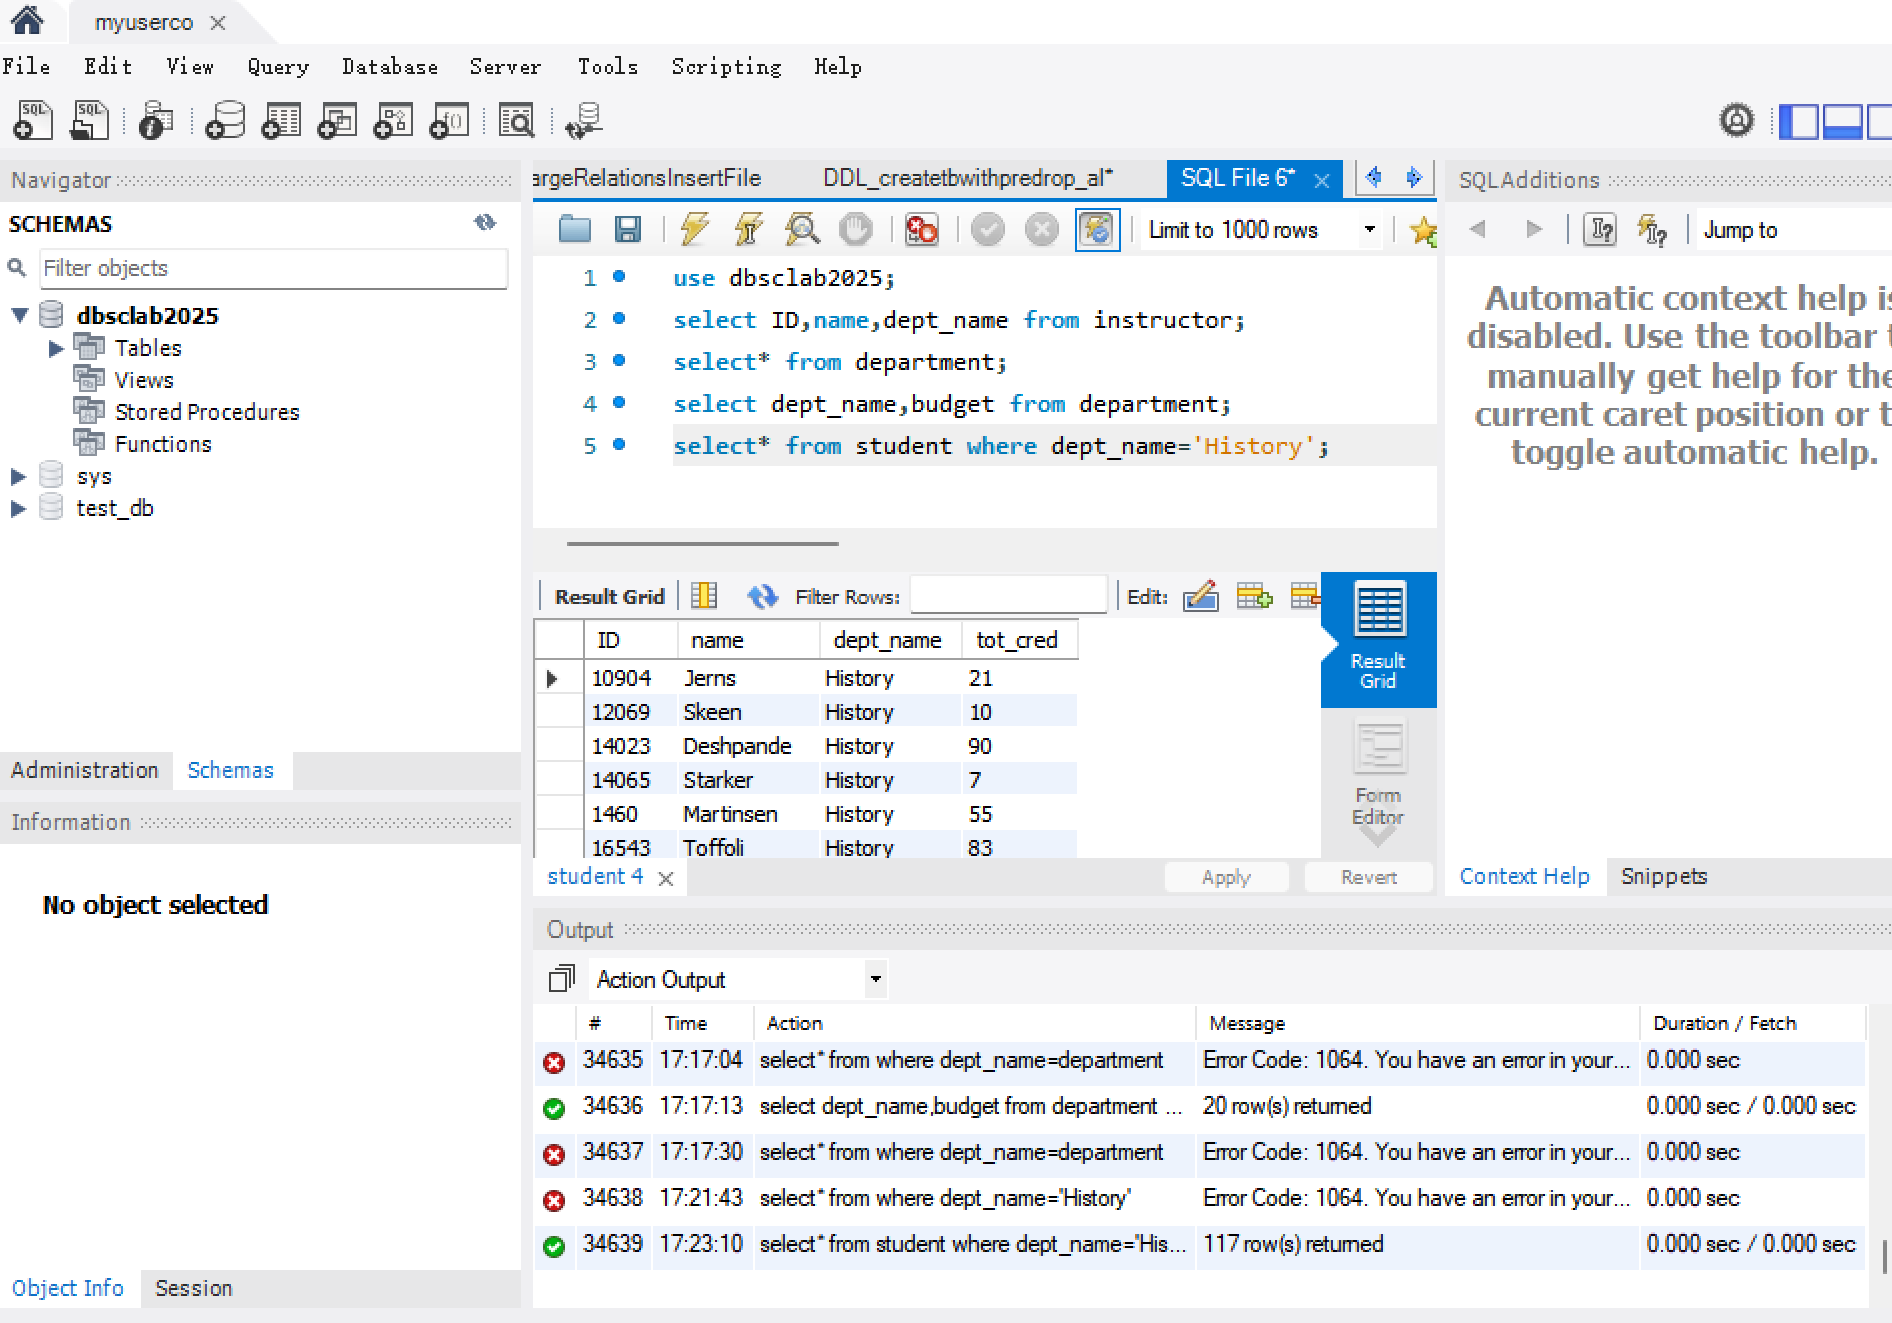
\includegraphics[width=12cm]{../figure/a0000-img018.png} \\
    \footnotesize 图18 数据操作查询截图16
\end{center}
\begin{center}
    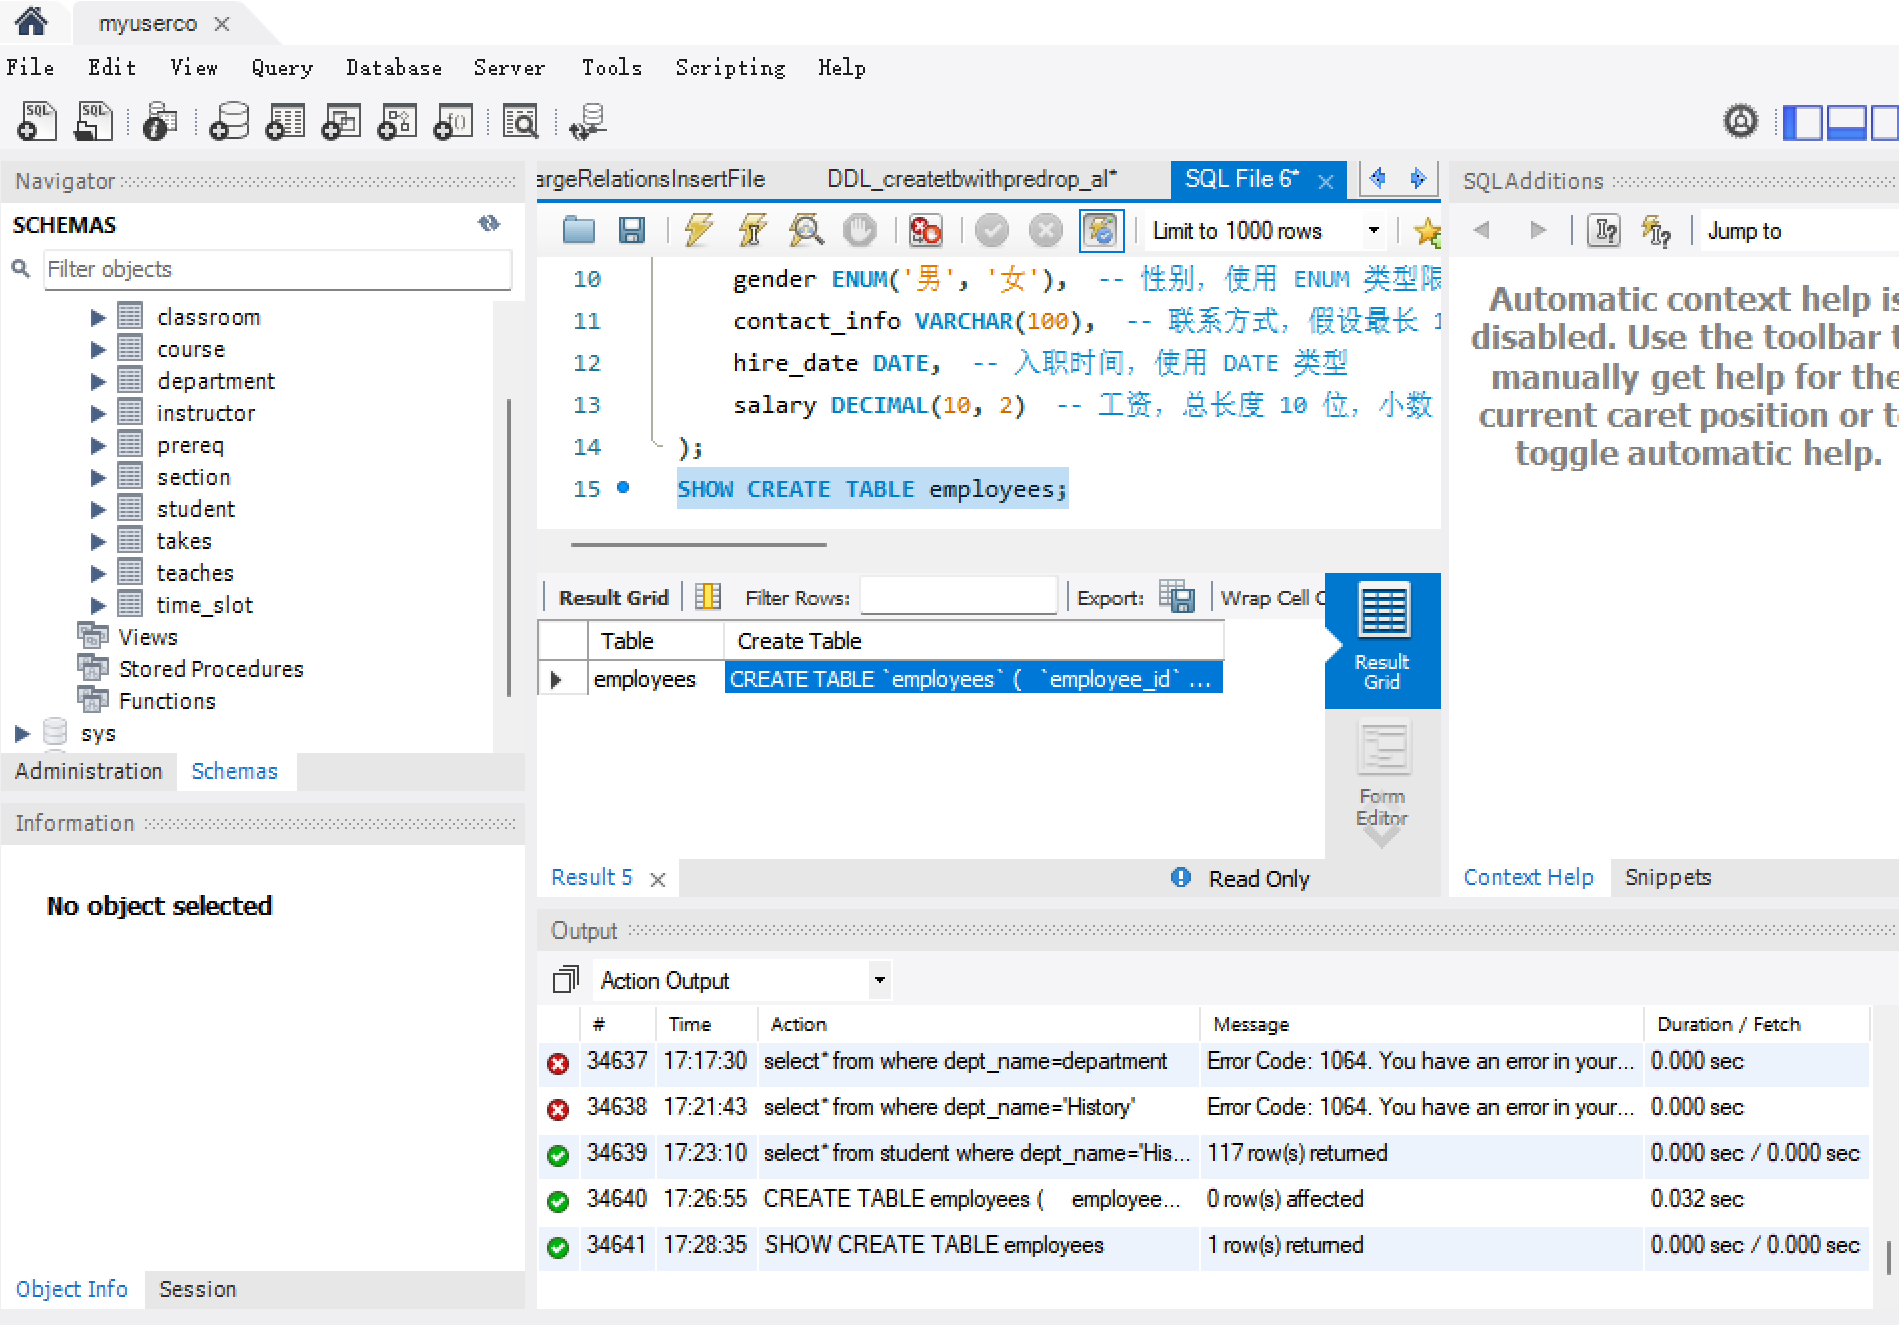
\includegraphics[width=12cm]{../figure/a0000-img019.png} \\
    \footnotesize 图19 数据操作查询截图17
\end{center}
\begin{center}
    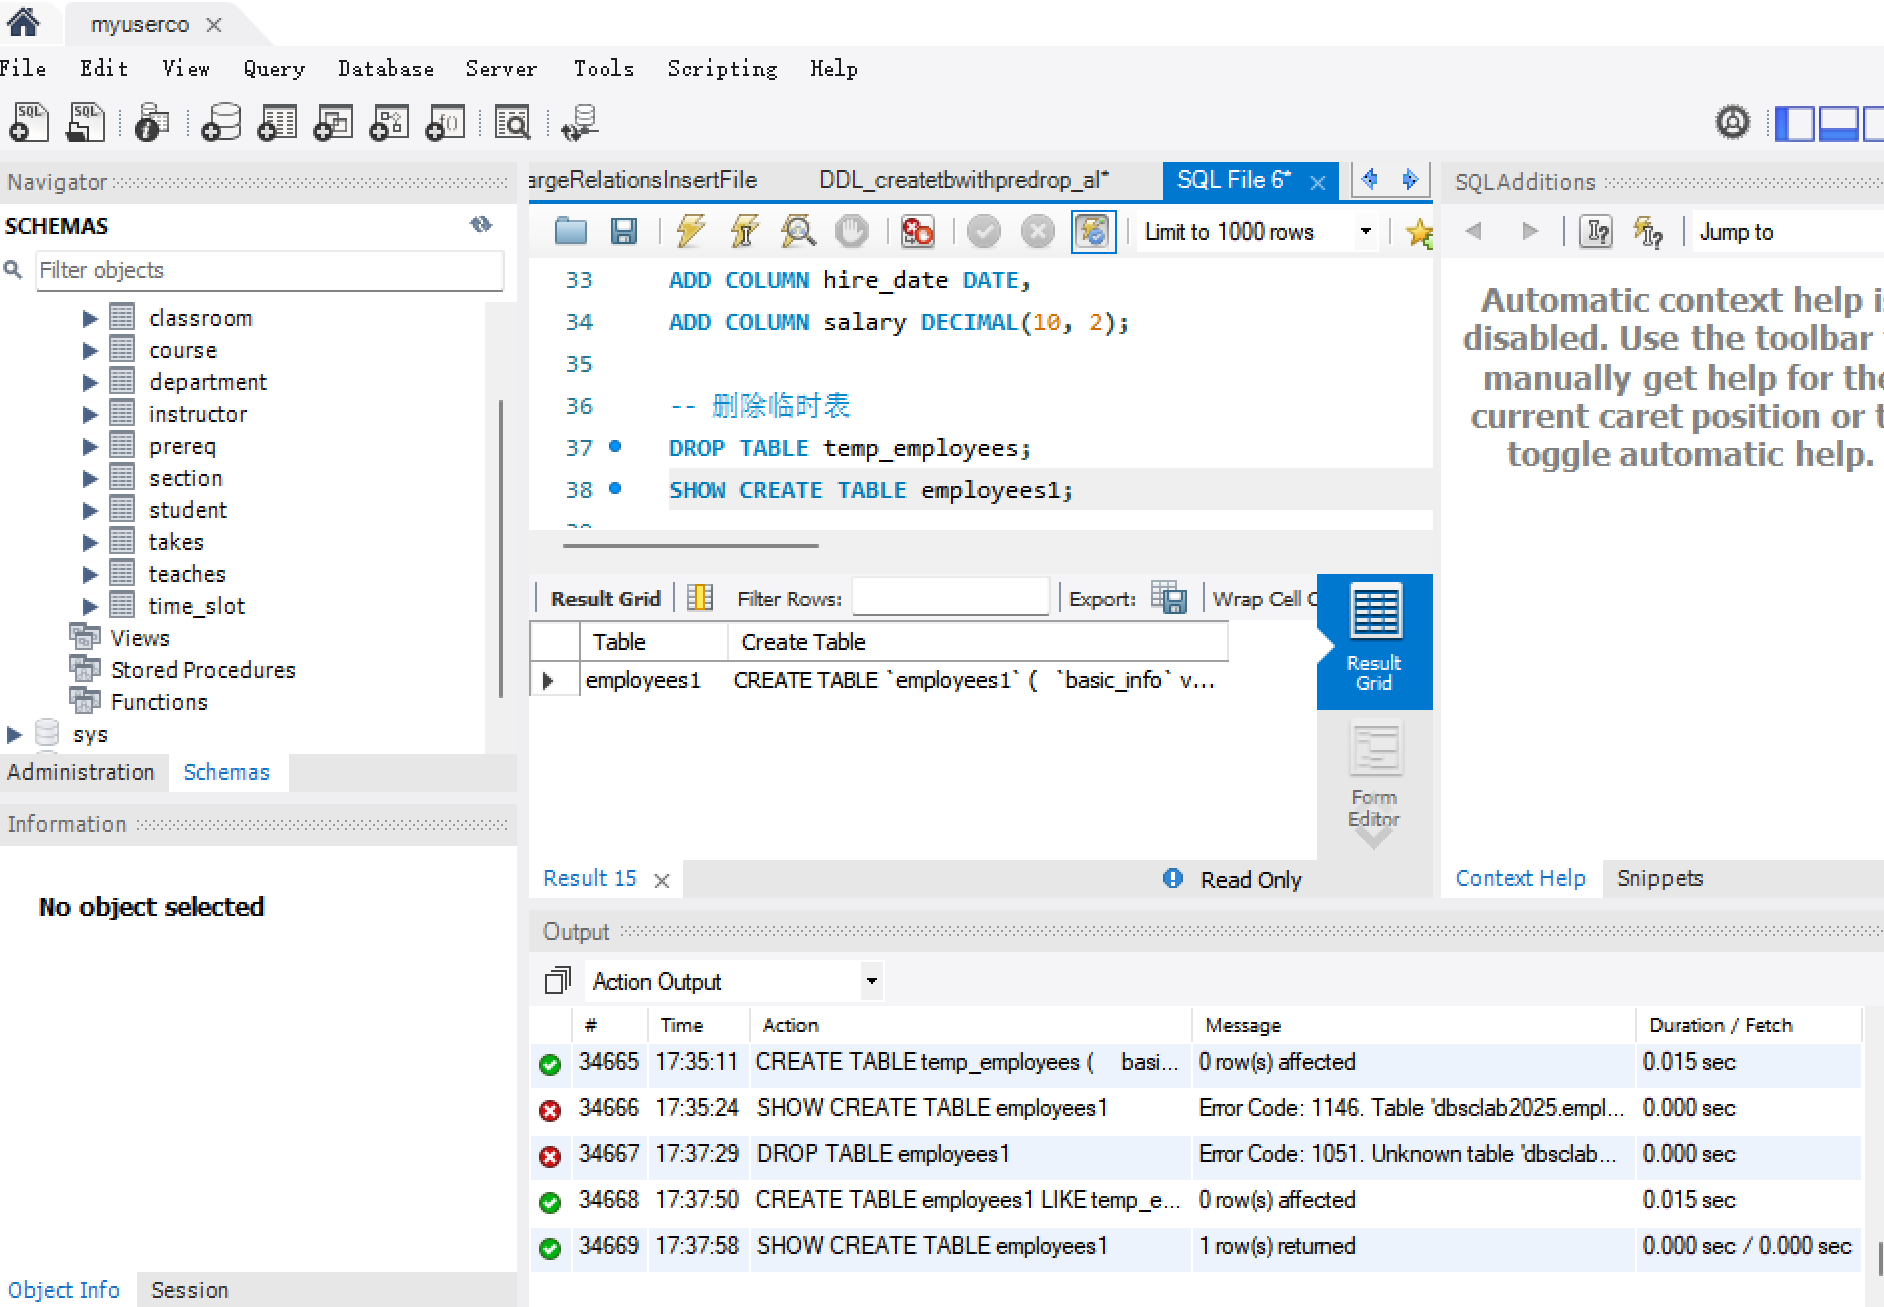
\includegraphics[width=12cm]{../figure/a0000-img020.png} \\
    \footnotesize 图20 数据操作查询截图18
\end{center}

\chapter{实验总结}
通过本次实验掌握了：
1. MySQL用户创建与权限管理
2. 数据库设计与数据导入
3. 复杂SQL查询编写
实验中遇到用户名输入错误问题，通过重新配置解决。熟悉了Workbench与Python结合使用的方法，为后续数据库开发奠定了基础。

\end{spacing}

\end{document}